\chapter{Обзор и анализ робототехнических систем, условия их применения}\label{ch:ch1}
Прежде чем разрабатывать робототехническую систему, необходимо проанализировать существующие решения которые используется в предполагаемых местах использования. Необходимо разобраться к какому семейству относится разрабатываемая система. На основе этой информации возможно избежать типичных проблем при разработке, связанных с конкретным типом движителя, которые неочевидны в начале разработки. 

Более того, необходимо просмотреть описания пещер, так как это является основным место для использования робототехнической системы. Знание препятствий, их размеров позволят подобрать параметры робота, максимально подходящие для обхода препятствий.

Любая робототехническая система не может обходиться без сенсоров. Поэтому необходимо рассмотреть существующее сенсоры, которые могут использоваться в мобильной робототехнике, предложить их классификацию и на основе классификации, выбрать необходимые сенсоры для решения поставленных задач. 

При разработке технической системы необходимо также рассмотреть алгоритмы навигации мобильных автономных роботов. 

После глубокого разбора всех систем, возможно объединить полученные знания и привести концептуальное решение, которое должно иметь возможность решить задачи разведки пещер.

\section{Классификация машин, использующих ноги в качестве движителя}
Эта классификация основана на работе \cite{Maloletov2015dinamica}. Первые попытки создания многоногих роботов были предприняты в эпоху до нашей эры. В настоящее время можно найти десятки конструкций шагающих роботов, но, как правило, это только экспериментальные прототипы. Из-за обилия различных конструкций, их классификация является нетривиальной задачей. Более того, термин <<ходьба>> имеет различные трактовки, что также является усложняющим фактором для классификации \cite{Bel1984,Brisk2009,Ohom1984,Pavl2013}. 

Определяющей особенностью аппарата, которая в целом позволяет говорить о шагании, является наличие специальных механизмов (ног, шагающих механизмов), которые обеспечивают движение аппарата в результате дискретного взаимодействия с опорой. Под дискретным взаимодействием понимают ситуацию, когда есть моменты времени, в которые механизм контактирует с опорной площадкой, и моменты времени, в которые с опорой механизм не взаимодействует.

Ходьба --- только один из нескольких возможных видов локомоции с помощью ног. Для двуногой системы: ходьба --- чередование опоры на одну ногу и опоры на обе ноги (потом на другую ногу); спортивная ходьба --- чередование опоры на одну ногу и на другую; бег --- чередование опоры на одну из ног и безопорного движения (потом на другую ногу); скачки --- чередование одноопорной, двухопорной и безопорной фаз; прыжки --- чередование опоры на обе ноги и безопорной фазы; прыжки на одной ноге - то же, что и прыжки, но одна нога вообще опоры никогда не касается.

Для многоногой системы понятие ходьбы легко обобщается. Спортивная ходьба и прыжки на одной ноге теряют смысл. А вот граница между бегом, прыжками и скачками уже не так очевидна \cite{Bel1984}. 

Если фаза движения машины с опорой на ноги чередуется с фазой покоя, в которой машина неподвижно лежит на опорной поверхности, то такое движение называется ползанием. Ноги могут быть оснащены специальными устройствами - захватами, присосками и т.п., позволяющими устройству осуществлять удерживающие связи с опорной поверхностью. Тип движения такого устройства называется лазанием.

Подводя итог, профессор Белецкий в своей книге использовал следующую классификацию. Важно отметить, что в одном экземпляре может сочетаться несколько типов движителей.

Псевдошагающие машины похожи на роботов с ногами, но их ноги всегда контактируют с опорной поверхностью. Другими словами, эти машины могут только имитировать полноценную походку. Одним из распространенных примеров является механическое устройство, называемая шагающий слон \pic{fig:mechEleph}.


\begin{figure}[H]
\centering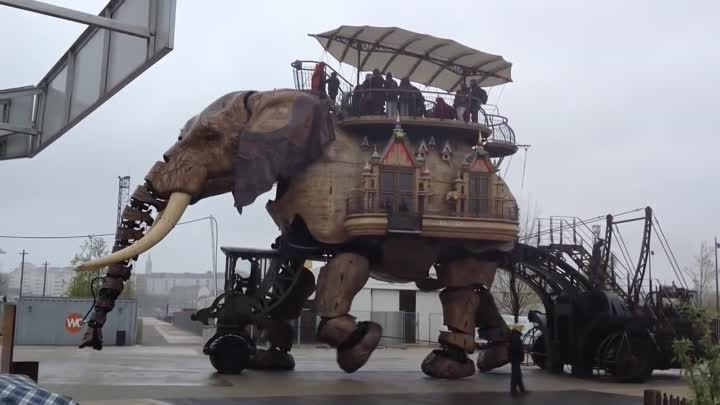
\includegraphics[width=0.8\textwidth]{from_master/mechEleph}
\caption{Механический слон}
\label{fig:mechEleph}
\end{figure}

К классу шагающих машин с дополнительными опорами относятся устройства, имеющие помимо дискретно взаимодействующих с опорной поверхностью шагающих движителей дополнительные механизмы, постоянно контактирующие с опорой \cite{Maloletov2015dinamica}. Необходимость в дополнительных опорах обычно возникает тогда, когда шагающих движителей недостаточно для обеспечения устойчивости машины. Чаще всего для этой цели шагающее транспортное средство оснащается колесной тележкой (рис. \ref{fig:Riksha},\ref{fig:steamMan})\cite{briskinSintezCiklovogoShagayushchego2011, Petr1986, Brisk2009,2014,2019,Pavl2013}.

\begin{figure}[H]
\centering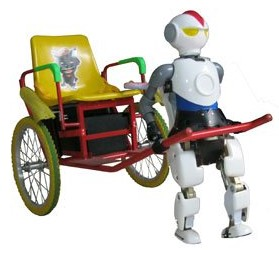
\includegraphics[width=0.6\textwidth]{from_master/Riksha}
\caption{Робот рикша}
\label{fig:Riksha}
\end{figure}

\begin{figure}[H]
\centering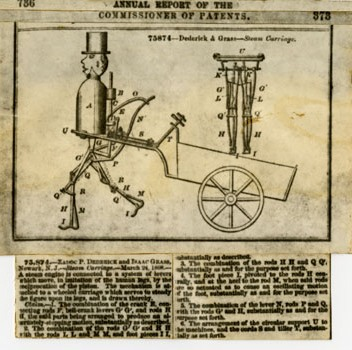
\includegraphics[width=0.9\textwidth]{from_master/steamMan}
\caption{Робот паровой человек}
\label{fig:steamMan}
\end{figure}

Такие машины обычно используются для демонстраций и отладки систем. Их применение бессмысленно, потому что они не обладают никакими преимуществами в сравнении с колесным роботом. 

Шагающие машины с циклическими движителями имеет несколько особенностей. Он характеризуется тем, что опорные точки шагающих механизмов движутся по одной и той же траектории относительно корпуса машины, и не решают проблемы адаптации к грунту и выбора точек постановки ног на землю. Такие машины имеют лучшую проходимость по сравнению с колесами меньшее сопротивление движению от земли, лучшее сцепление с основной поверхностью, большие возможности для снижения давления на грунт \cite{cruse2001control}. Примеры машин с циклическими движителями: (рис. \ref{fig:chebishev},\ref{fig:kuban}).

\begin{figure}[H]
\centering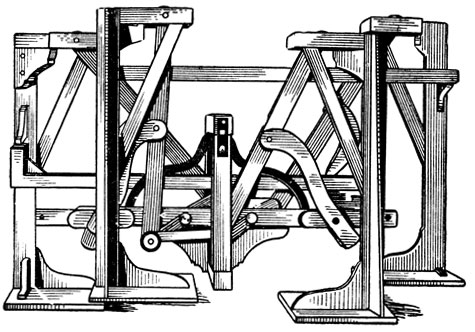
\includegraphics[width=0.8\textwidth]{from_master/chebishev}
\caption{Машина Чебышева}
\label{fig:chebishev}
\end{figure}

\begin{figure}[H]
\centering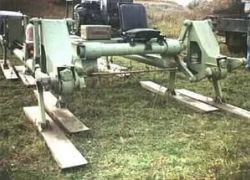
\includegraphics[width=0.9\textwidth]{from_master/kuban.jpg}
\caption{Робот ВолгГТУ Кубань}
\label{fig:kuban}
\end{figure}

Главной особенностью циклических шагающих машин является их простота конструкции и управление. 

Полноценная ходьба --- модификация предыдущего типа движителя и она дает наибольшие преимущества по сравнению с другими заявленными типами движителей. 

Данный способ передвижения позволяет использовать произвольный закон изменения скорости движения ноги как на этапе взаимодействия с землей, так и на этапе переноса. Такие машины обычно превосходят традиционные транспортные средства не только по грунтовой, но и по профильной проходимости. А их главным недостатком является сложность конструкции и системы управления. Это самый разнообразный и многообразный класс шаговых машин в мире, и многие из приведенных здесь примеров относятся к этому классу. 

Колесно-шагающими машинами традиционно называют класс устройств, в которых колеса шагающих движителей служат упорами. Такие машины могут работать в двух режимах: в режиме колесной машины и в режиме шагающей машины. В первом случае машина движется только с помощью колес. Во втором случае машина совершает шагающие движения, отрывая поочередно колеса от земли и переставляя их на новое место. В этом случае те, что соприкасаются с землей, могут либо блокироваться, либо поворачиваться в соответствии с движением опорных ног.
Известно несколько примеров (рис. \ref{fig:vniitm},\ref{fig:alduro},\ref{fig:athlete}) \cite{germann2001joystick}.

\begin{figure}[H].
\centering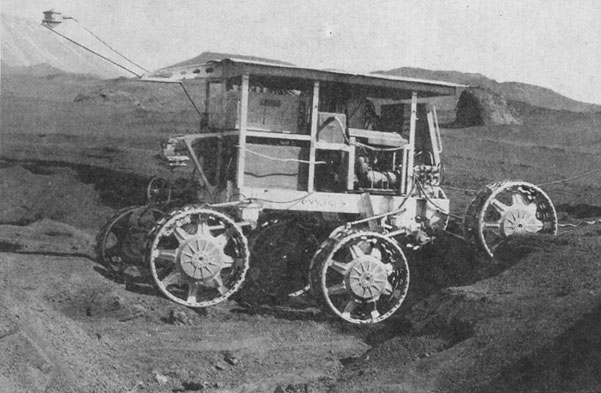
\includegraphics[width=0.9\textwidth]{from_master/vniitm}
\caption{VNIITM}
\label{fig:vniitm}
\end{figure}

\begin{figure}[H]
\centering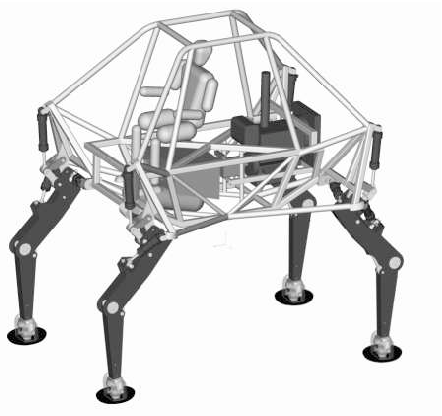
\includegraphics[width=0.9\textwidth]{from_master/alduro}
\caption{Робот Alduro}
\label{fig:alduro}
\end{figure}

\begin{figure}[H]
\centering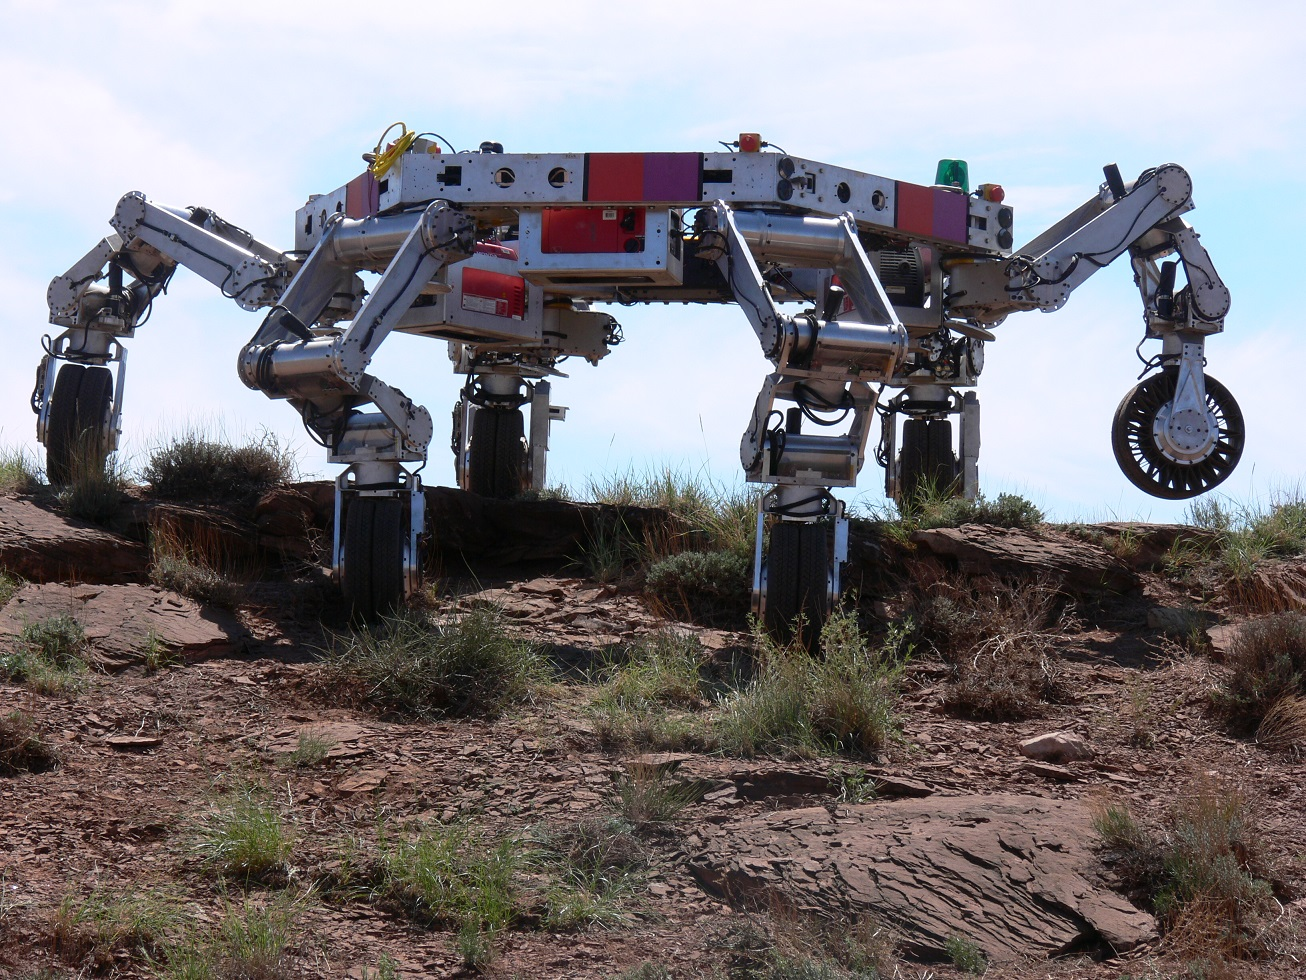
\includegraphics[width=0.8\textwidth]{from_master/athlete}
\caption{Робот Athlete}
\label{fig:athlete}
\end{figure}

Есть несколько моашин, которые могут не только прыгать или бегать, но и шагать. Примеры следующие \cite{Pavl2013,volkovaModelirovanieDvizheniyaMnogozvennogo2013,bidgoly2010learning,yacunVibrorobotDlyaVertikalnogo2010} \pic{fig:bigDog}.

\begin{figure}[H]
    \centering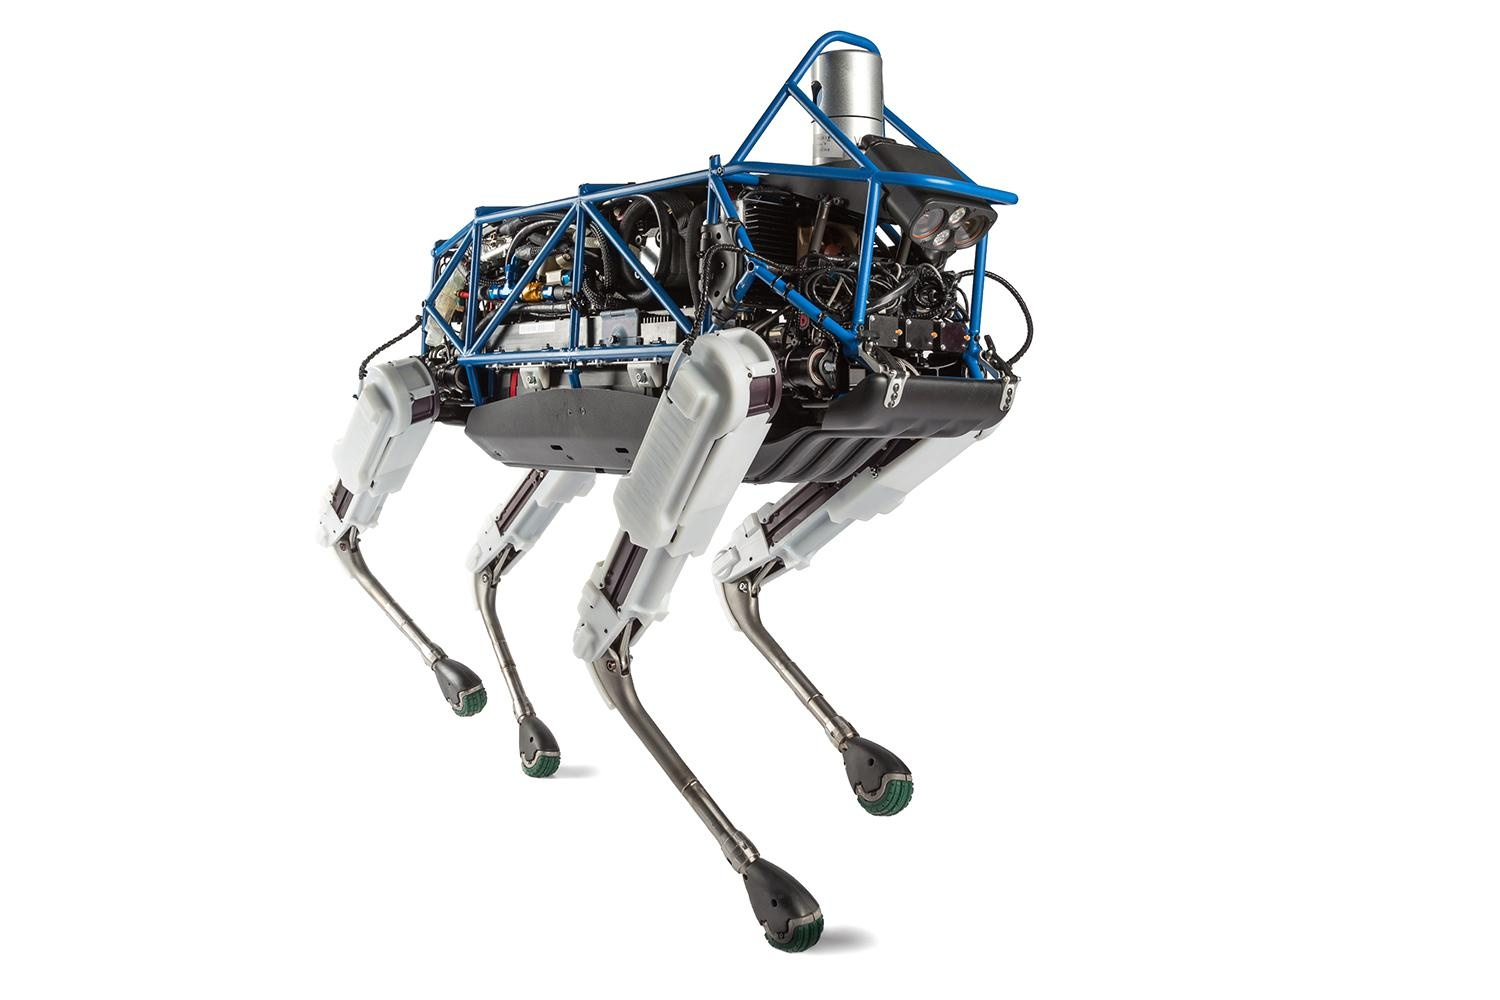
\includegraphics[width=0.9\textwidth]{from_master/bigDog}
\caption{BigDog}
\label{fig:bigDog}
\end{figure}

В соответствии с определением выше, к ползающим экскаваторам относится большинство таких машин, как шагающие экскаваторы \pic{fig:Esh6}. Несмотря на название "шагающие", такие машины перемещаются, поднимаясь по лестнице и ложась на опору при передвижении ног \cite{peters2010prototype,gradeckiySostoyaniePerspektivyRazvitiya2014,bidgoly2010learning}.

\begin{figure}[H]
\centering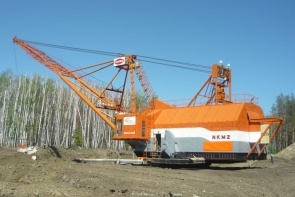
\includegraphics[width=0.8\textwidth]{from_master/Esh6}
\caption{Ползающий экскаватор Российского производства}
\label{fig:Esh6}
\end{figure}

 Специфика взаимодействия с опорной поверхностью и область применения лазающих машин настолько сильно отличаются, что сравнение их показателей (за исключением общетехнических) становится практически бессмысленным. Следует также отметить, что многие ползающие и лазающие роботы не имеют ног или какого-то их подобия, передвигаясь, например, за счет движений гибкого тела.

\begin{figure}[H]
\centering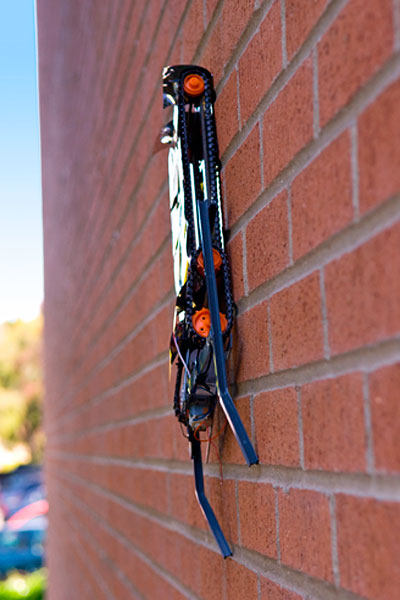
\includegraphics[width=0.45\textwidth]{from_master/brickwall}
\caption{BrickWall робот}
\label{fig:brickwall}
\end{figure}

\begin{figure}[H]
\centering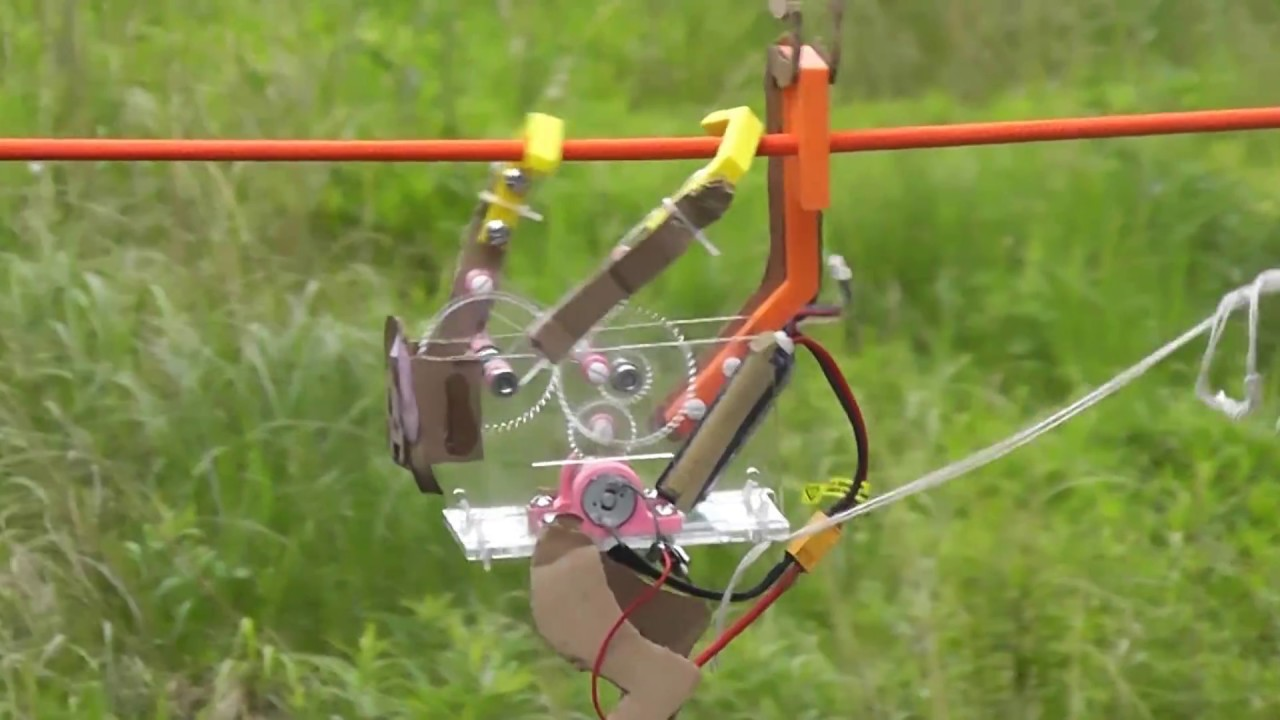
\includegraphics[width=0.8\textwidth]{from_master/ropeClimbing}
\caption{Робот, взбирающийся по канату}
\label{fig:ropeClimbing}
\end{figure}

Согласно этой классификации, робот, который используется в экспериментальной части, относится к категории <<Шагающие машины с циклическим действием движителей>>.

В течении разработки робототехнической системы, были спроектированы и изготовлены несколько прототипов шагающих роботов. Первым всемирно известным прототипом с подобной системой движения является робот RHex \cite{saranliRHexSimpleHighly2001} от Boston Dynamics. Группы ученных по всему миру развивали эту идею. Таким образом появились 3 новых подмножества. Роботы, которые умеют много сочленений. Системы, которые могут трансформироваться в колесных роботов и обратно. А также системы, которые являются псевдоколесными, то есть количество ног на одном моторе больше одной. Как итог, было решено добавить сочленение в разрабатываемую конструкцию. Также было оценен концепт с псевдоколесными роботами, так как это увеличивает проходимость по грунтам.

\section{Роботы, которые могут использоваться для исследования пещер}

Как было отмечено выше, одной из основных областей применения разрабатываемых роботов являются пещеры. Исследование пещер естественного происхождения является комплексной задачей, сопряженная со множественными трудностями \cite{Zhang2017a, Frumkin2019}. Деградация сенсоров \cite{Huang2019}, перебои в коммуникации между роботами из-за потери сигналов \cite{Vaquero2018, Thangavelautham2017}, сложный рельеф пещер \cite{Thangavelautham2017}, обилие грязи \cite{Baker2004}, жидких препятствий \cite{Morris2006}, требующие герметизацию корпуса, являются только малой частью встречаемых проблем в пещерах. 

В пещерах возможно встретить почти все типы поверхностей, с которыми приходится сталкиваться роботам в мире. Это и твердые поверхности: мрамор, кварц, базальт. Осадочные горные породы, такие как: мел, гипс, известняк. Часто встречаются водные препятствия — как лужи, так и целы залы, погруженные в воду. Особую опасность для человека вносят сифоны. Скользкие поверхности: лед, мох, глина, а так же разрушаемые поверхности — каменная гряда и паутина \cite{1960,1963,1969,1971}. Знание типов поверхностей и габаритов пещер влияет на типы сенсоров, которые будут установлены на робота и на на необходимую автономность робототехнической системы \cite{Mascarich2018a}. 

Для преодоления сложного рельефа различные роботы, робототехнические системы и типы движителей были предложены исследователями по всему миру \cite{Morris2006a}. Разрушение пещер нежелательно, поэтому роботы, которые для перемещения ломают породу, не рассмотрены в данном обзоре \cite{Semini2016}. Для исследования пещер используются, как наземных роботов, так и летающие аппараты, робототехнические комплексы. Из летающего транспорта это коптеры \cite{Papachristos2019,Scaramuzza2014,zinggMAVNavigationIndoor2010} и дирижабли \cite{Huang2019}. Дирижабль намного более автономен и может нести большую нагрузку. Наземных роботов очень много типов, но основными являются: шагающие \cite{Tan2016,Lynch2019} колесные \cite{Molyneaux2016,Vaquero2018}, трековые \cite{Reddy2015} и специфичные. Специфичные движители это движители роботов, которые не поддаются классификации, например змеевидные \cite{Ye2007,Borenstein2007}, шарообразные \cite{Thangavelautham2017,Dubowsky2008,Dang2019} и другие.

Для исследования пещер система роботов является самым эффективным способом разведки. Для использования систем роботов необходимо решать дополнительные задачи, как архитектурного характера, телекоммуникационного и управленческого. Обычно системы состоят из нескольких одинаковых роботов \cite{Vaquero2018}, связка – коптер и шагающий \cite{Chen2010,Cantelli2013}.

Ползающие роботы \cite{Schmidt2013} являются перспективными для исследования пещер по причине их высокой проходимости по узким и невысоким лазам. Например, известны ползающие роботы для исследования пещер, находящихся на других планетах \cite{Parness2017}. 

Важным критерием для выполнения задач разведки пещер, является способность перемещаться по вертикальным поверхностям, благодаря высокой адгезии с поверхностью. Это достигается следующими способами: существуют магнитный \cite{Lee2012,tavakoliOmniClimberOmnidirectionalLight2012,Kotay1996,Xu2017}, электрический \cite{Li2017}, негативного давления \cite{Lee2012,tavakoliOmniClimberOmnidirectionalLight2012,Papachristos2019}, пневматический или помощью присосок \cite{Nagakubo1994,Tlale2012}, зацепов ("когтей"), что иногда называют механической адгезией \cite{Parness2017,Bretl2006,SangbaeKim2005,Sintov2011}. Последний способ является самым применимым для пещер, так как стены рельефные. Рельефные стены с одной стороны препятствуют другим способам прикрепления к поверхности, а с другой стороны облегчают использование зацепов.

Навигация в пещерах является нетривиальной задачей, поэтому рассмотрены сенсоры и алгоритмы, а также архитектурные решения, которые используются в представленных выше роботах. Целесообразно рассмотреть работы в близких и смежных областях. К примеру, исследование трубопровода \cite{Savin2017} или завалов после техногенных катастроф. С точки зрения навигации основной проблемой является недостаток света, а также сильная неоднородность территории и обилие гранулированных поверхностей. Решение данной проблем сейчас уделено много внимания, одним из подтверждений данного тезиса является прошедшее соревнование DARPA Subterranean Challenge. В данном направлении используются как лазерные дальномеры (лидары), так и визуальные SLAM алгоритмы \cite{Mascarich2018a,Dang2019a,Fairfield2006,Chhaniyara2012}. С точки зрения архитектуры, наблюдается тенденция к модульности, а также к возможным защитам от потерь робота \cite{Miller2019,weiStudyMineRescue2009}. при работе роботов в группе один робот был потерян, то остальные роботы все равно должны передавать друг другу данные. 

Очень важно уметь правильно передвигать робота по сыпучим грунтам, следующие работы посвящены этим проблемам \cite{Tan2016,Savin2017,Chhaniyara2012,Tsounis2019, Li2009,Bjelonic2019,DeViragh2019,Buchanan2019}. Критичным критерием навигации является решение задачи в реальном времени.

Тип опорной поверхности является одним из ключевых параметров для адоптации управления робота. Зная тип опорной поверхности возможно оптимально построить маршрут по исследуемой территории. Следующие статьи и их обзоры покрывают основные способы решения данной задачи \cite{wuIntegratedGroundReaction2016,wuTactileSensingTerrainBased2020,luo_robotic_2017}.

Подведя итог, в данном разделе были представлены причины проблем, возникающие при разведке пещер роботами. Представлены причины, к примеру типы опорных поверхностей, которые влияют на подбор сенсоров и алгоритмов, а также сделаны выводы как это влияет на робототехническую систему. После этого показаны решения, предложенные исследователями по всему миру, связанные с навигацией, подбором движителя, выбором сенсоров и архитектурными решениями, дающие надежную систему. 

\section{Исследования роботов с цикловым движителем}
Одной из разновидностью роботов с цикловым движителем является гексаподы. Гексапод это разновидность мобильных шагающих роботов с 6 конечностями. Такая форма демонстрирует качественное поведение сороконожки. То есть, чаще всего роботы гексаподы --- биомиметические роботы, то есть роботы, вдохновленные природой.

Не смотря на это, существуют интересные попытки создать гибриды между колесными роботами и многоножками, чтобы получить <<лучшее из обоих миров>>.

Boston Dynamics RHex \cite{Altendorfer2001} - это шестиногий робот \pic{fig:rhex}. Данный робот является идейным вдохновителем множества разработок по всему миру, в том числе и для робота, разработанного автором диссертации. Независимо управляемые ноги создают специальные походки, которые перемещают его по неровной местности, такой как лестница, каменная гряда и т.д. Данный робот умеет прыгать. Форма ног обеспечивает плавность движений. Однако у робота есть и ряд недостатков. Прежде всего, это высокое энергопотребление, так как он содержит шесть двигателей. Кроме того, у этого робота есть некоторые трудности с управляемостью. 

\begin{figure}[H]
    \centering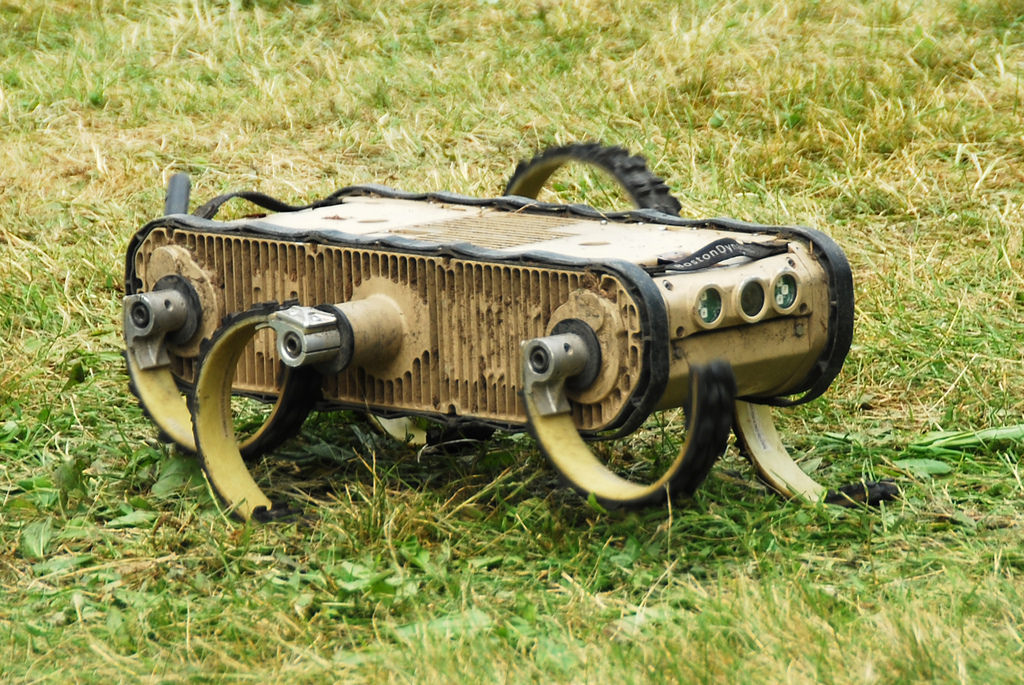
\includegraphics[width=0.9\textwidth]{from_master/rhex}\\
    \caption{Boston Dynamics робот RHex}
    \label{fig:rhex}
    \end{figure}

Gakken Mechamo Centipede \cite{millerExtremeMakeoverHeianera2008, Miller2019} - робот \pic{fig:gakken}, который имеет схожую кинематическую схему с СтриРусом. Стрирус это разработанный автором робот. Большое количество ног может обеспечить ему хорошую проходимость на пересеченной местности, и потеря ноги не будет критичной для робота. Однако это увеличило количество компонентов робота, что удорожает производство и техническое обслуживание. Минусом данной конструкции это малая длина педипулятора снижает возможности передвижения по пересеченной местности.
\begin{figure}[H]
    \centering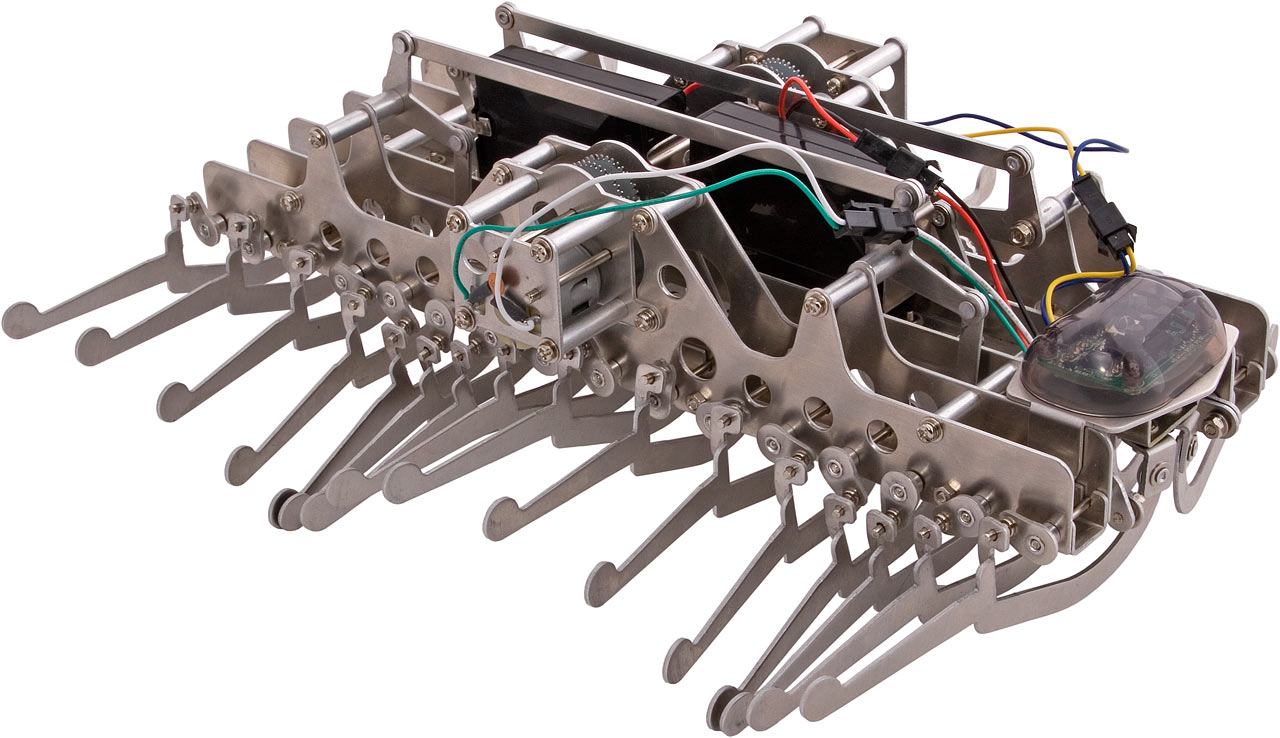
\includegraphics[width=0.8\textwidth]{from_master/gakken}\\
    \caption{Gakken Mechamo Centipede робот}
    \label{fig:gakken}
    \end{figure}

Quattroped и TurboQuad \cite{shenDesignLegwheelHybrid2009, Chen2014, Chen2017} --- это роботы, трансформирующие колеса в ноги \pic{quatro}. Когда он использует ноги, его кинематическая схема похожа на робота RHex, в случае режима работы колес он похож по управлению представляет собой четырёхколёсное транспортное средство. Данный инженерный прием обеспечивает высокую скорость на ровной местности, но конструкция робота становится конструкционно сложной, что снижает надежность системы. У робота 4 ноги, что делает его неустойчивым в некоторых ситуациях.

\begin{figure}[H]
    \begin{subfigure}{0.99\textwidth}
    \centering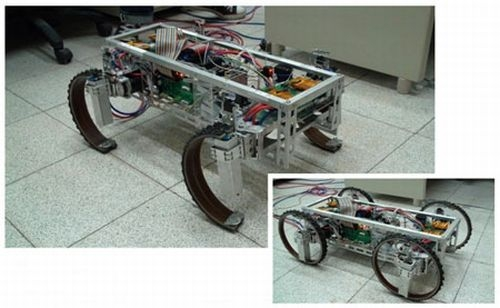
\includegraphics[width=0.9\textwidth]{from_master/quattroped}\\
    \caption{Quattroped robot}
    \label{fig:quattroped}
    \end{subfigure}

    \begin{subfigure}{0.99\textwidth}
    \centering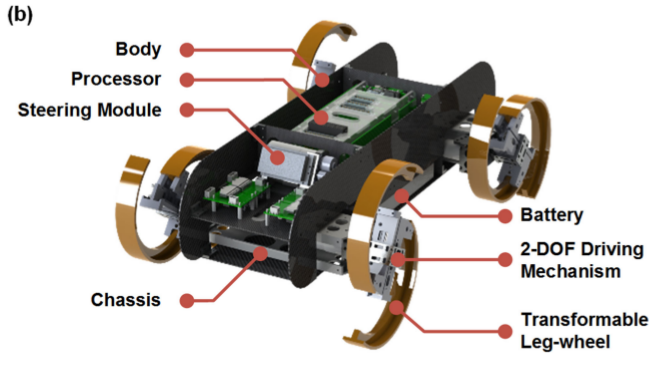
\includegraphics[width=0.9\textwidth]{from_master/turboquad}\\
    \caption{TurboQuad robot}
    \label{fig:turboquad}
    \end{subfigure}
    \caption{Quattroped семья роботов}
    \label{quatro}
    \end{figure}

Whegs \cite{schroerComparingCockroachWhegs2004} \pic{fig:whegs} использует стратегию локомоции, которая сочетает простоту колеса с преимуществами преодоления препятствий ногой. Робот обладает сегментированным телом, что позволяет ему при малой длине педипуляторов соперничать по проходимости с остальными представителями данного класса роботов. Сегментированность корпуса делает робота более сложным в изготовлении и управлении.

\begin{figure}[H]
\centering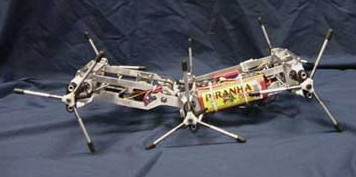
\includegraphics[width=0.9\textwidth]{from_master/whegs2.jpg}\\
\caption{Whegs II}
\label{fig:whegs}
\end{figure}

Сравнительный анализ между представленными выше роботами приведен в таблице \ref{tabular:robot_comparison}.
\begin{table}[H]
    \centering
\caption{Сравнительный анализ гексаподов}
\label{tabular:robot_comparison}
% \small
\begin{tabular}{l|c|c|c|c}
\toprule
\toprule
\rowcolor{Gray}
 Параметры, СИ & RHex & \makecell{Gakken \\ Mechamo\\ Centipede} &  \makecell{Quattroped} & \makecell{Whegs II}\\
 \hline
Длина, мм & 540 & 320 & 600 & 470 \\ 
  \rowcolor{LightGray}
 Ширина, мм & 200 & 140 & 190 & 360 \\
 Высота, мм & 127 & 100 & 140 & 50 \\
  \rowcolor{LightGray}
 Масса, кг & 8.2 & 1.1 & 8.6 & 3.86 \\ 
 Количество ног & 6 & 32 & 4 & 18 \\
  \rowcolor{LightGray}
 Высота ноги, мм & 175 & 50 & 175 & 100  \\
 Масса ноги, кг & 0.1 & 0.02 & 0.38 & 0.05 \\
  \rowcolor{LightGray}
 Скорость, м/с & 1.6 & 0.1 & 2 & 1.5 \\
\bottomrule
\bottomrule
\end{tabular}
% \end{center}
\end{table}

Все эти роботы, кроме Gakken Centipede, были созданы для разведки, в том числе и пространствах искусственного происхождения, поэтому значения параметров можно легко объяснить. Ширина должна быть меньше ширины дверного проема. Еще лучше, если ширина робота будет меньше 2/3 размера двери, и все прототипы удовлетворяют этому условию. При навигации внутри помещений длина также должна быть минимально возможной, иначе он не сможет передвигаться в коридорах и тесных помещениях. Масса зависит от других параметров. Высокая скорость не нужна в помещениях и опасных зонах. 

Роботы с цикловым движителем, такие как Boston Dynamics RHex \cite{Altendorfer2001}, Gakken Mechamo Centipede \cite{Miller2019}, Quattroped and TurboQuad \cite{Chen2011,Chen2014,Chen2017}, а так же Whegs \cite{schroerComparingCockroachWhegs2004} были рассмотрены. Рассмотрев других представителей выбранного класса роботов и определив причины таких параметров, было решено, что не следует превышать длину аппарата в один метр, в ширину --- меньше 70 см (стандартная ширина дверного проема). Иметь меньше 32 лапок и высота лапки должна быть больше 10 см. При большем количестве лапок начинаются большие проблемы с трением и кпд, что негативно сказывается на проходимости и энергопотреблении конструкции.


\section{Описание условий в пещерах}
Пещера -- полость в верхней части земной коры, сообщающаяся с поверхностью одним или несколькими входными отверстиями. Пещеры естественного происхождения бывают: карстовые, тектонические, эрозионные, ледниковые и вулканические. В них могут быть найдены следующие структуры поверхностей:
\begin{itemize}
    \item твердые породы, прочные -- мрамор, кварц, базальт (магма) \pic{fig:solid_surfaces};
    \item твердые породы, поддатливые -- мел, гипс, соль, известняк \pic{fig:solid_surfaces};
    \item сыпучие грунты -- песок, глина, снег \pic{fig:running_soils};
    \item водные преграды -- как и лужи (малый слой воды), залы, погруженные под воду, сифоны \pic{fig:water_obstacles};
    \item скользкие поверхности -- отложения мха и плесени, лед \pic{fig:slippery_surfaces};
    \item разрушаемые поверхности -- каменная гряда, паутина.
\end{itemize}


\begin{figure}[H]
\begin{subfigure}{0.49\textwidth}
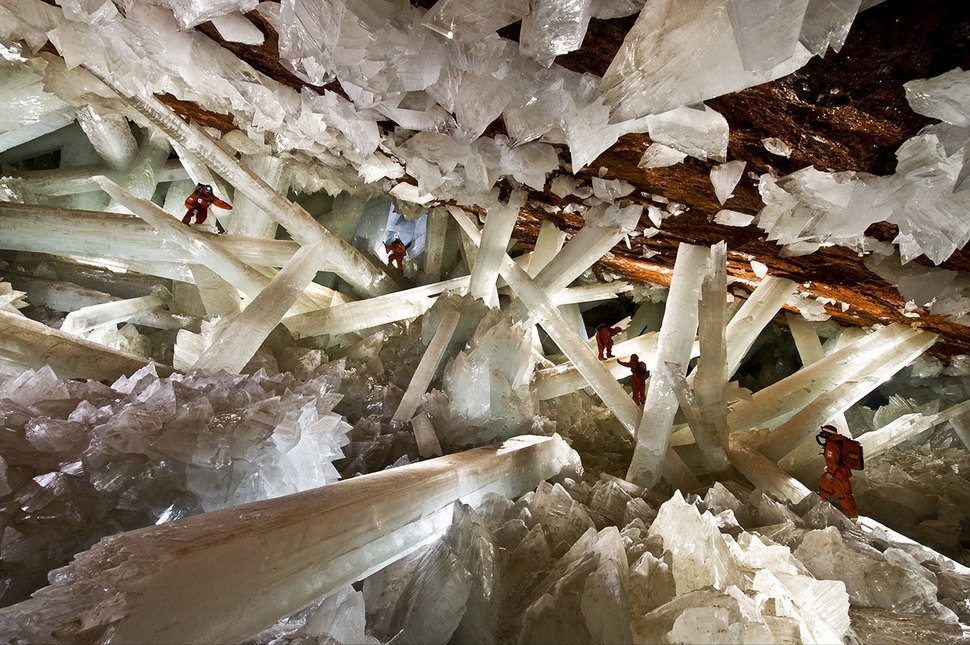
\includegraphics[width=0.99\textwidth]{surface_types/crystal.png}\\
\caption{Кристаллы}
\label{fig:crystal}
\end{subfigure}
\begin{subfigure}{0.49\textwidth}
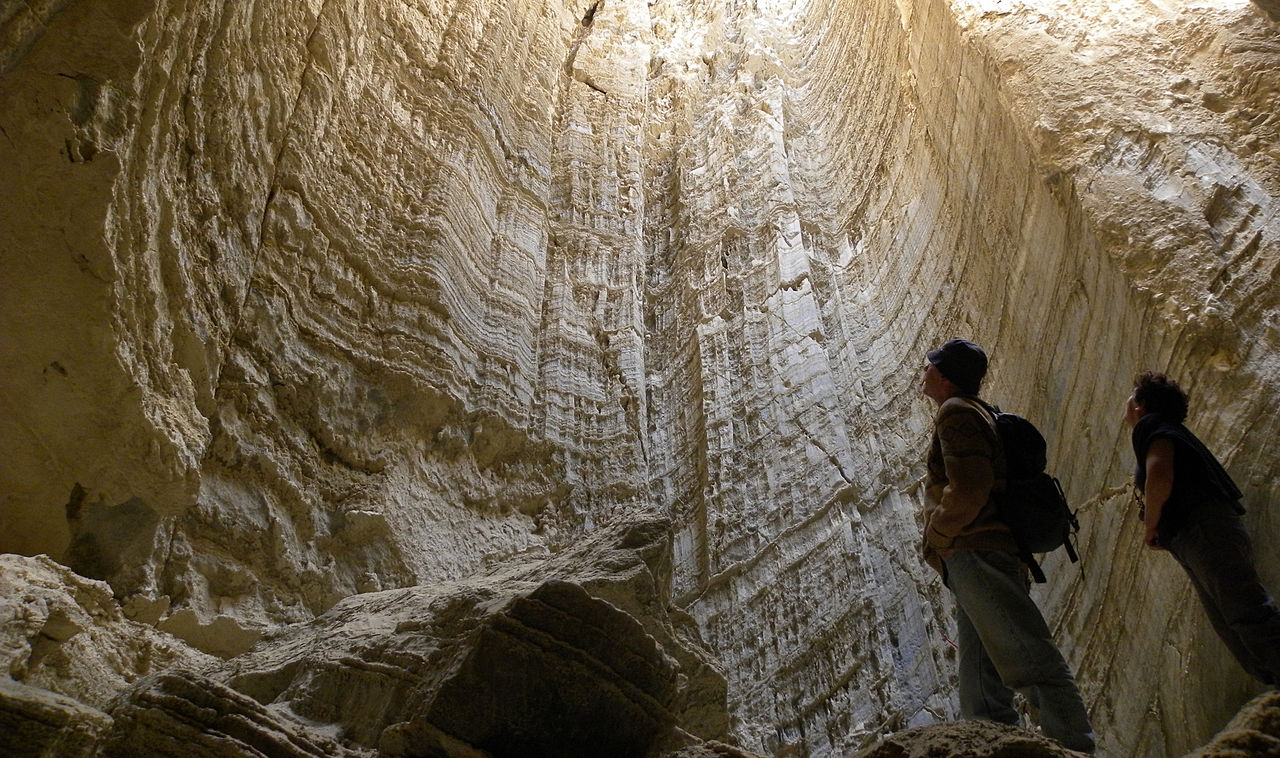
\includegraphics[width=0.99\textwidth]{surface_types/salt.jpg}\\
\caption{Солевые отложения}
\label{fig:salt}
\end{subfigure}

\begin{subfigure}{0.49\textwidth}
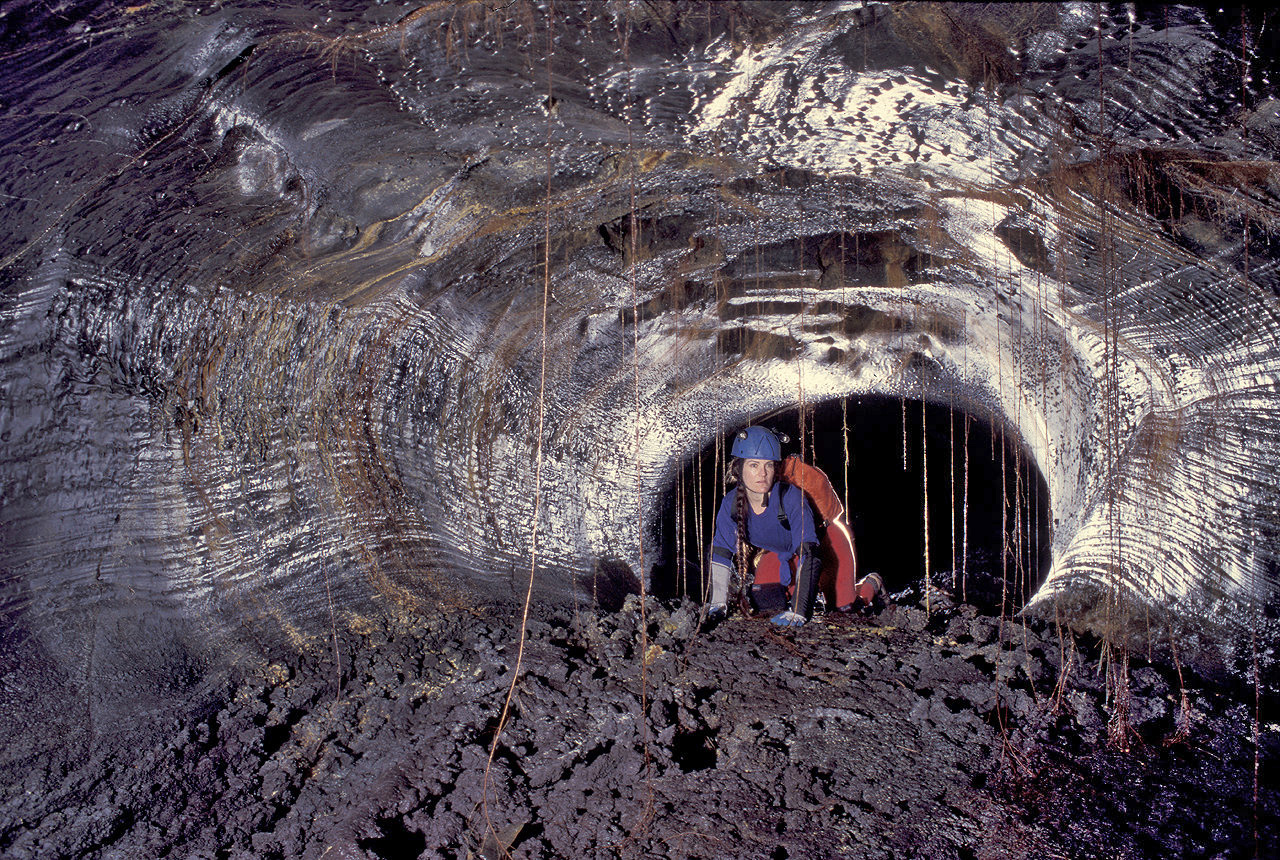
\includegraphics[width=0.99\textwidth]{surface_types/lava.jpg}\\
\caption{Магма}
\label{fig:lava}
\end{subfigure}
\begin{subfigure}{0.49\textwidth}
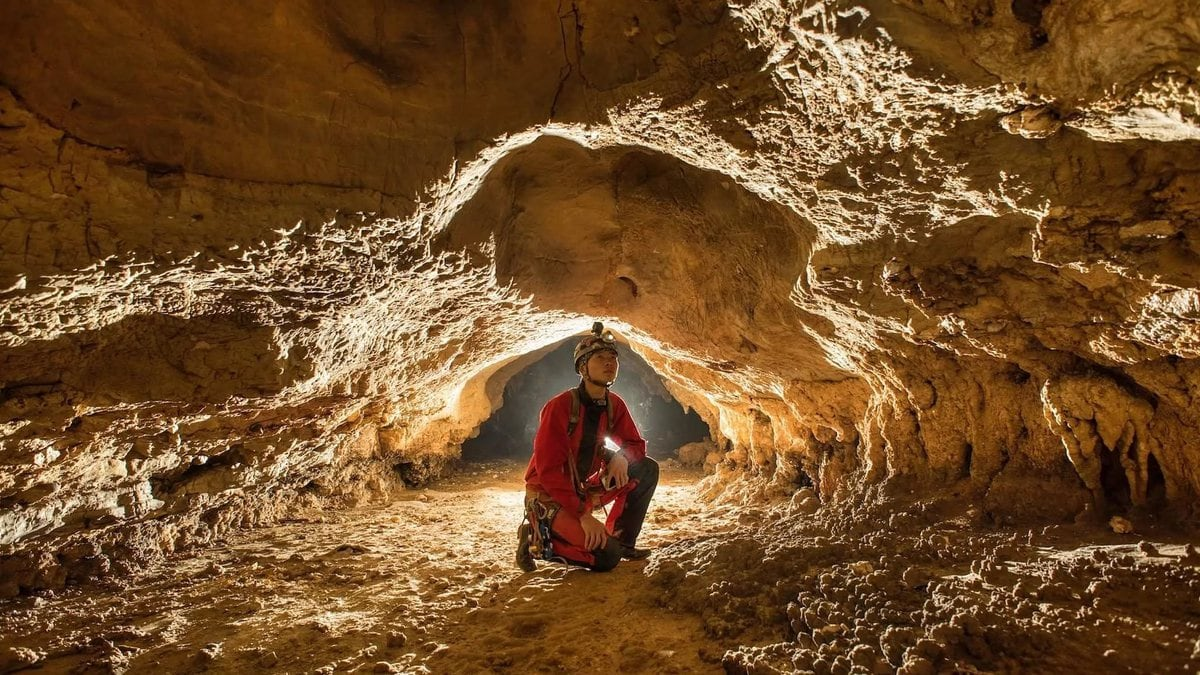
\includegraphics[width=0.99\textwidth]{surface_types/limestone.png}\\
\caption{Известняк}
\label{fig:limestone}
\end{subfigure}
\caption{Твердые поверхности}
\label{fig:solid_surfaces}
\end{figure}

\begin{figure}[H]
\begin{subfigure}{0.49\textwidth}
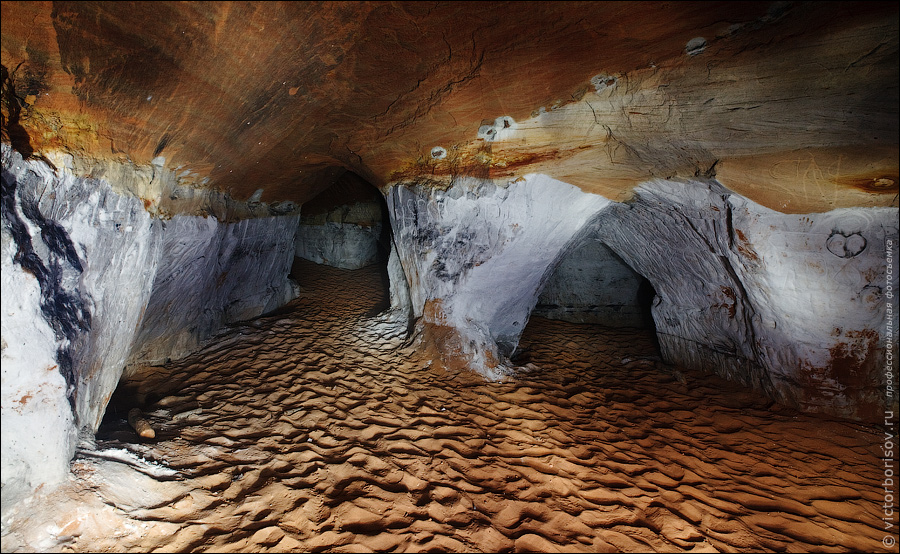
\includegraphics[width=0.99\textwidth]{surface_types/sand.jpg}\\
\caption{Песок}
\label{fig:sand}
\end{subfigure}
\begin{subfigure}{0.49\textwidth}
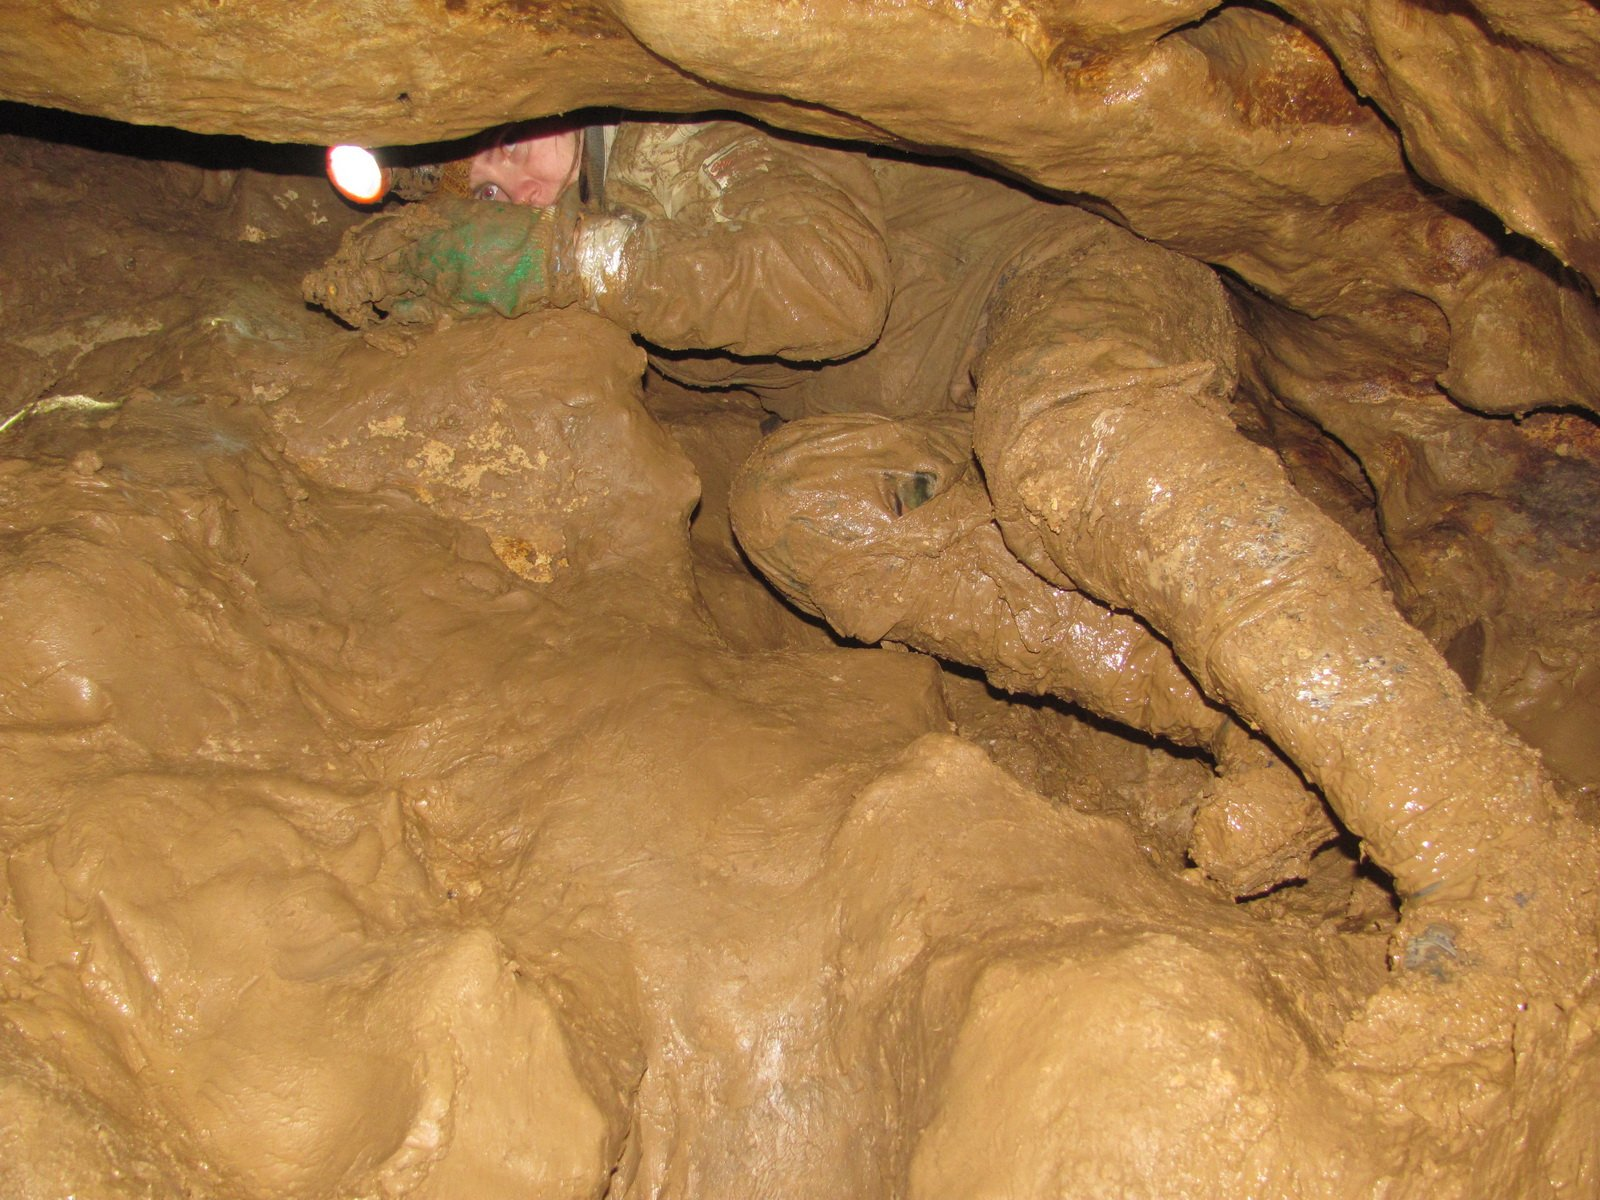
\includegraphics[width=0.89\textwidth]{surface_types/clay.jpg}\\
\caption{Глина}
\label{fig:clay}
\end{subfigure}
\caption{Сыпучие грунты}
\label{fig:running_soils}
\end{figure}

\begin{figure}[H]
\begin{subfigure}{0.49\textwidth}
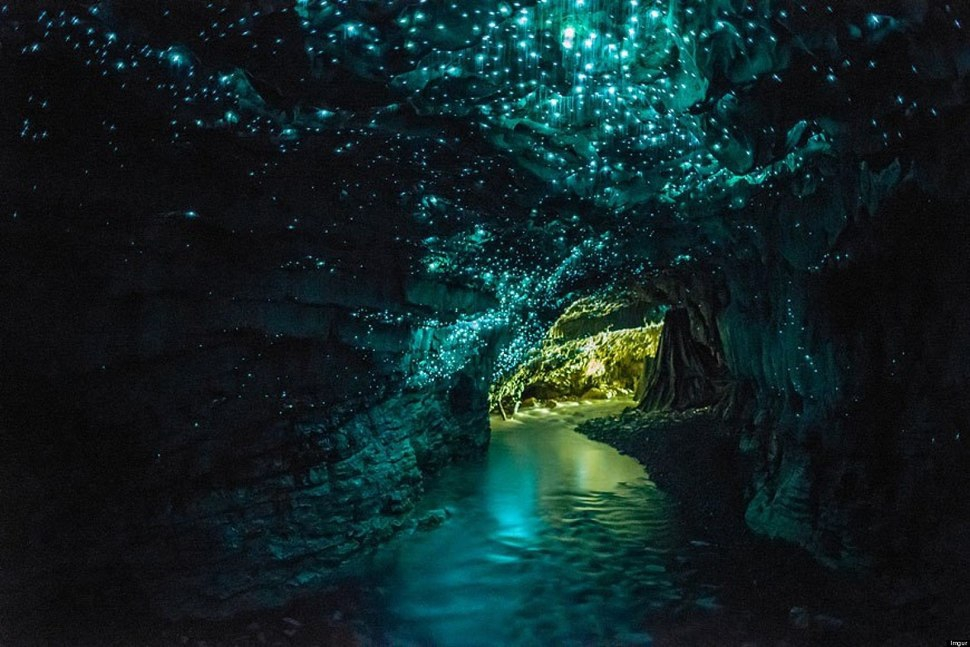
\includegraphics[width=0.99\textwidth]{surface_types/splash.png}\\
\caption{Лужа}
\label{fig:splash}
\end{subfigure}
\begin{subfigure}{0.49\textwidth}
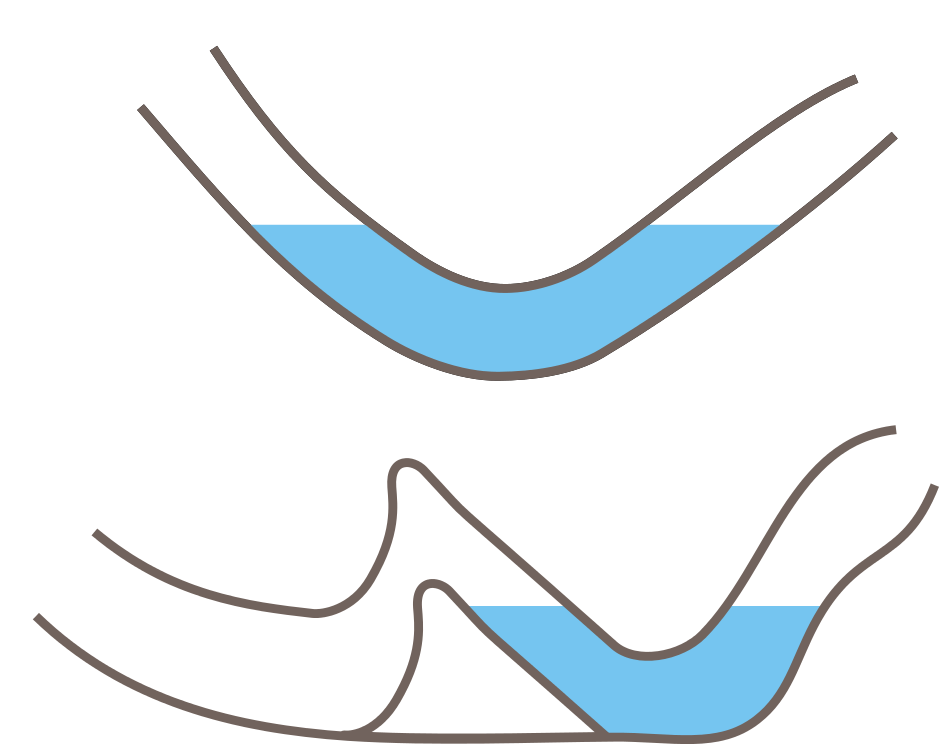
\includegraphics[width=0.84\textwidth]{surface_types/siphon.png}\\
\caption{Сифон}
\label{fig:siphon}
\end{subfigure}
\caption{Водяные препятствия}
\label{fig:water_obstacles}
\end{figure}

\begin{figure}[H]
\begin{subfigure}{0.49\textwidth}
\centering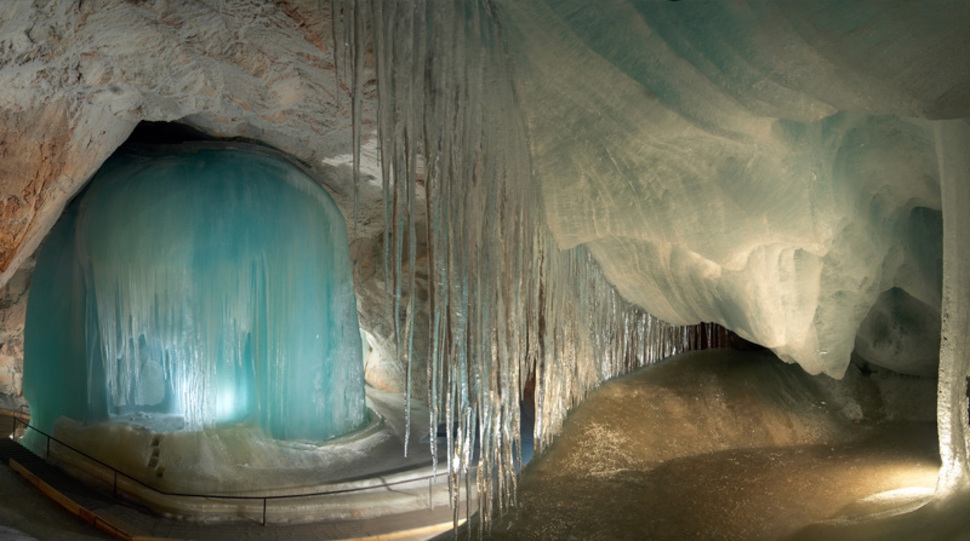
\includegraphics[width=0.99\textwidth]{surface_types/ice.png}\\
\caption{Ледяная пещера}
\label{fig:icee}
\end{subfigure}
\begin{subfigure}{0.49\textwidth}
\centering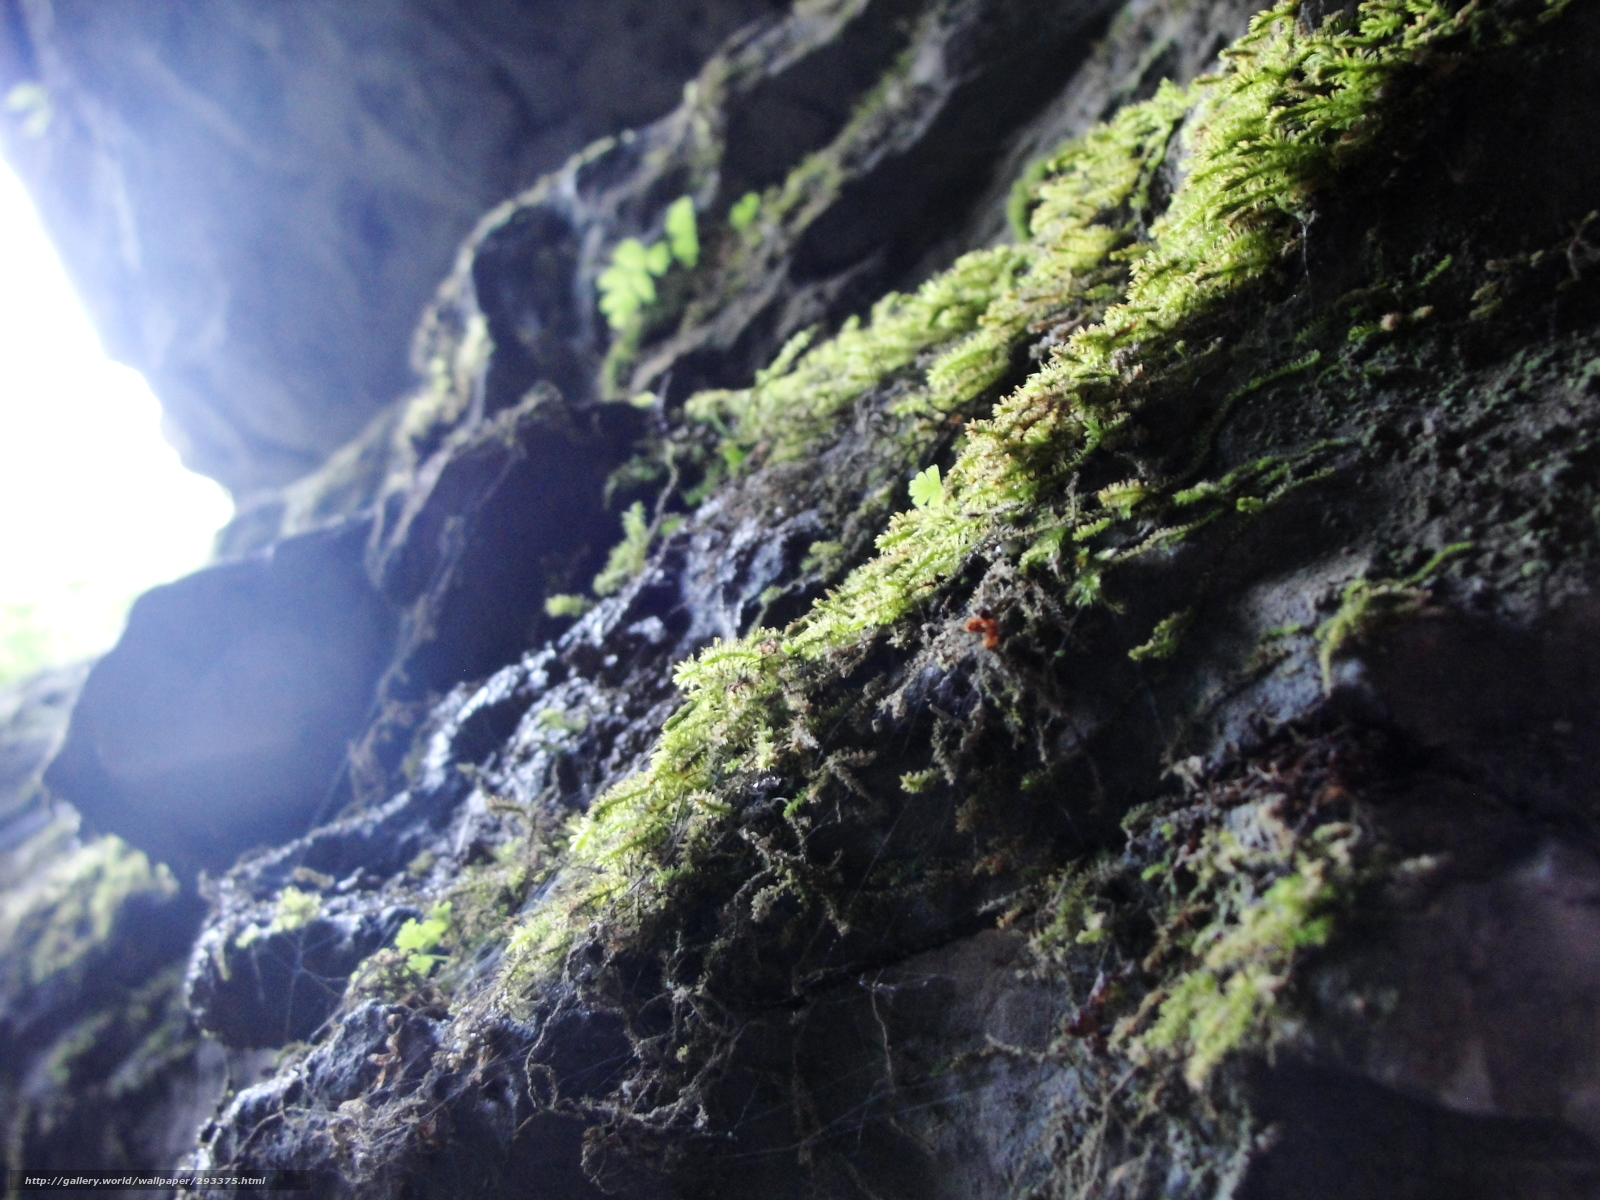
\includegraphics[width=0.99\textwidth]{surface_types/moss.jpg}\\
\caption{Мох}
\label{fig:moss}
\end{subfigure}
\caption{Скользящие поверхности}
\label{fig:slippery_surfaces}
\end{figure}

Представлены габаритные размеры нескольких пещер для определения необходимого запаса хода и размеров компонентов робототехнического комплекса \cite{1960,1963,1969,1971}.

\begin{figure}[H]
\begin{subfigure}{0.8\textwidth}
\centering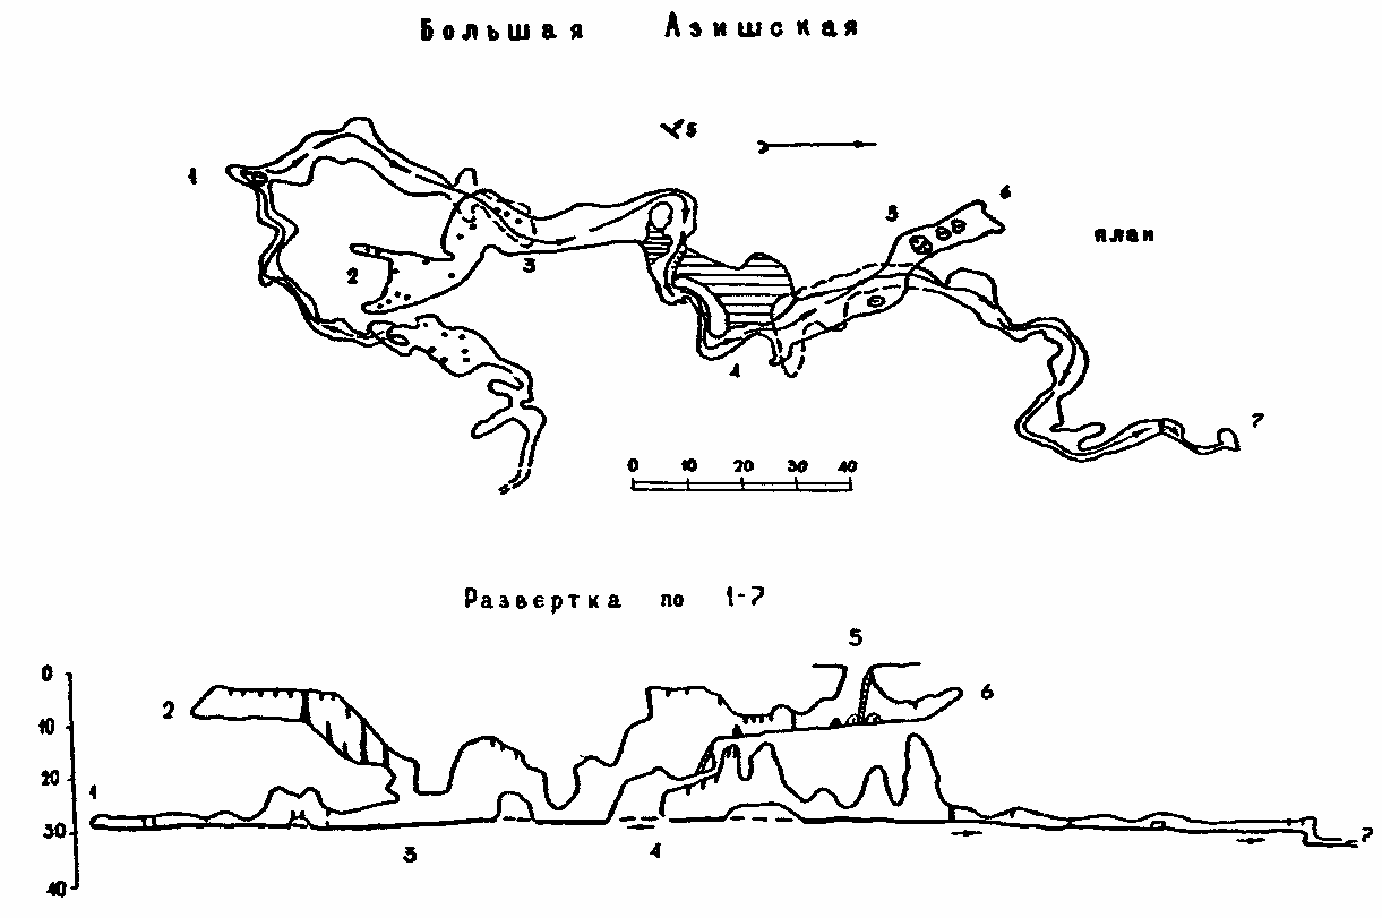
\includegraphics[width=0.7\textwidth]{cave_maps/map1.png}\\
\caption{Большая Азишская пещера}
\label{fig:ice}
\end{subfigure}

\begin{subfigure}{0.8\textwidth}
\centering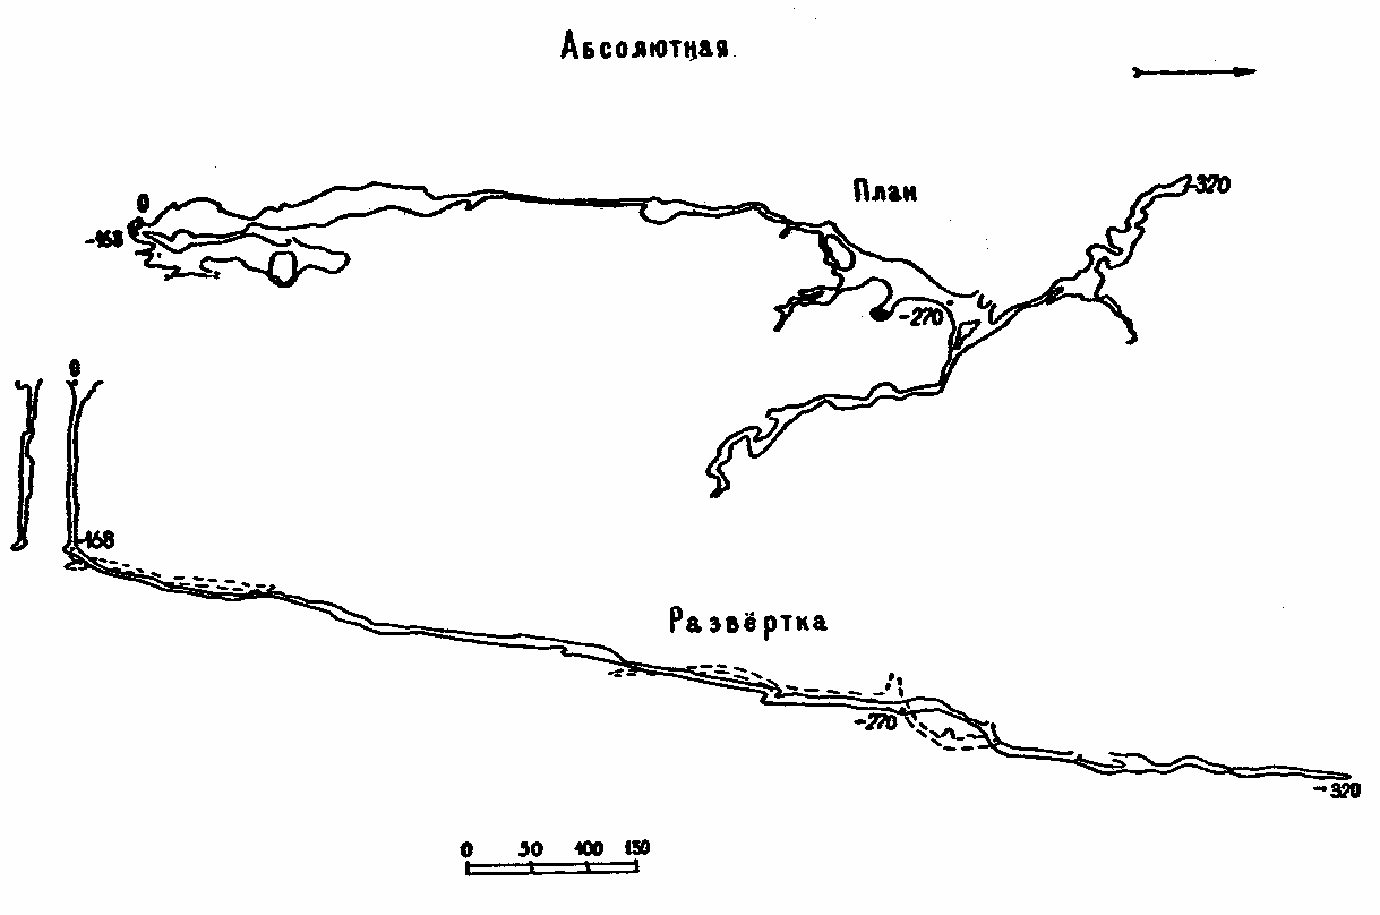
\includegraphics[width=0.7\textwidth]{cave_maps/map2.png}\\
\caption{Абсолютная пещера}
\end{subfigure}

\begin{subfigure}{0.8\textwidth}
\centering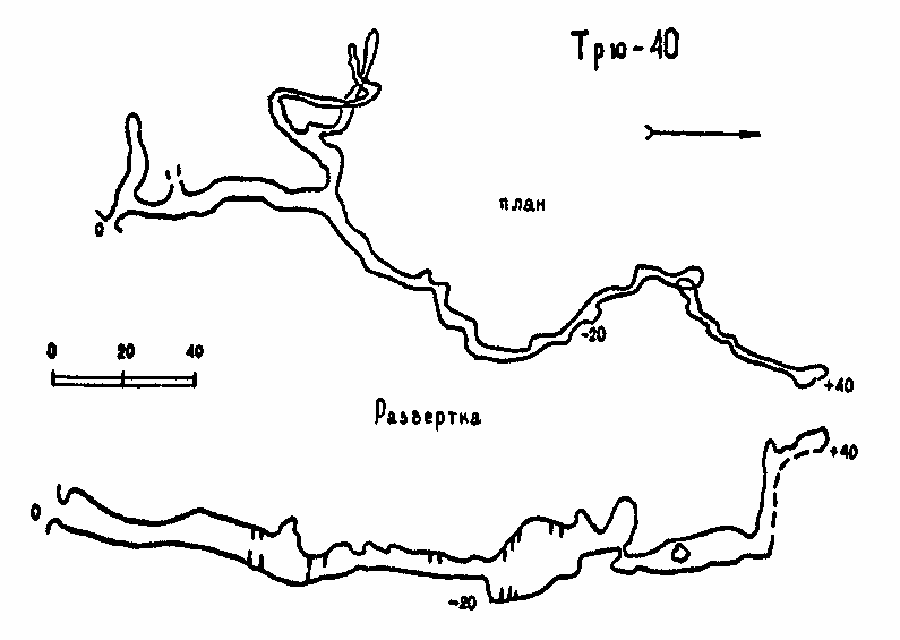
\includegraphics[width=0.7\textwidth]{cave_maps/map3.png}\\
\caption{Трю - 40}
\end{subfigure}
\caption{Примеры карт некоторых пещер}
\end{figure}

Так как существующие карты построены только там, где прошли исследователи-люди, то таким образом возможно только оценить верхние границы для габаритов робота. Основное преимущество робота это то, что он может пройти в те места, которые недоступны человеку из-за своих размеров.


\section{Классификация сенсорных устройств}
Информация, поступающая с различных сенсорных устройств, используется в системе управления робота для обнаружения и распознавания объектов внешней среды, построения модели окружающих поверхностей, а также для управления движением робота и его манипуляторов при выполнении различных технологических операций. В соответствии с этим, используемые в роботах предложенного класса, группы сенсорных устройств можно описать как сенсоры, необходимые для выявления свойств внешней среды, отдельных объектов и обеспечения перемещения исполнительных органов \cite{2013,1984,2015}.

К первой из указанных групп относятся сенсорные устройства, предназначенные для выявления различных физико-химических свойств объектов среды, включая, в частности, устройства для выявления параметров рельефа в рабочей зоне мобильных роботов, специальных признаков для обнаружения и распознавания определенных объектов, положения и их ориентации в рабочей зоне относительно робота и т. п.

Ко второй группе относятся датчики обратной связи (положения, скорости, ускорения), усилий, возникающих при взаимодействии робота с внешней средой, прикосновения, проскальзывания и т. д.

Такое разделение сенсорных устройств достаточно условно, поскольку, например, сенсорные устройства первой группы могут быть использованы и для определения положения захвата манипулятора робота в рабочей зоне, т. е. играть роль датчиков обратной связи при управлении движением.

Сенсорные устройства робота могут воспринимать информацию на различных расстояниях от ее источника. По этому признаку сенсорные устройства делятся на сверхближние, ближние, дальние и сверхдальние (работающие вне рабочей зоны).

Сенсорные устройства сверхближнего действия используют для очувствления захватов и других частей манипуляторов, а также корпуса робота. Они позволяют фиксировать их контакт с объектами внешней среды (тактильные датчики), измерять усилия, возникающие в месте взаимодействия (силометрические датчики), фиксировать проскальзывание объектов.

Сенсорные устройства ближнего действия обеспечивают получение необходимой информации в непосредственной близости от робота, но бесконтактным способом. К таким устройствам относятся локационные сенсоры захвата, неконтактные бамперы, различные дальномеры ближнего действия, плотнометры грунта и т. п. Бесконтактные измерительные устройства технически сложнее контактных, но позволяют роботу выполнять задание с большей скоростью, заранее получать информацию о ближайших объектах и соответствующим образом корректировать свои действия.
Сенсорные устройства дальнего действия дают информацию о внешней среде и объеме всей рабочей зоны робота.

Сенсорные устройства сверхдальнего действия применяют главным образом в мобильных роботах. К таким устройствам относятся различные навигационные устройства, координаторы, локаторы и другие оптические, радиотехнические и телевизионные системы.

В бесконтактных сенсорных системах роботов для получения требуемой информации могут быть использованы излучаемые таким устройством специальные сигналы (оптические, радиотехнические, радиационные и т. п.) или естественные излучения среды и отдельных ее объектов. В зависимости от этого различают активные и пассивные сенсорные системы. Первые обязательно включают передающие устройства, излучающие первичный сигнал, и приемные устройства, регистрирующие прямой сигнал, прошедший через среду, или вторичный сигнал, отраженный от объектов среды. Пассивные системы имеют только приемное устройство, а роль излучателя играют сами объекты внешней среды. Поэтому такие устройства технически обычно проще и дешевле, но зато и менее универсальны. Существуют также полуактивные сенсорные устройства, в которых в результате излучения внешней среды инициируется вторичное излучение ее объектов, принимаемое приемными устройствами, как в пассивных системах.
 
Таким образом, на основе классификации были выбраны следующие сенсоры для решения задач перемещения и локализации в пещерах, параллельно определяя тип опорной поверхности. Выбранными семействами сенсоров являются силомоментные, сверхдальнего действия, бесконтактные, а также датчики обратной связи.

\section{Обзор подходов оценки поверхностей}Генерация семейства поверхностей является одним из способов решить задачу оценки сложности рельефа. Основными найденными подходами к оценке рельефа являются.
\begin{enumerate} 
    \item Анализ множества физических свойств поверхностей с точки зрения максимальной скорости, мощности и других параметров робота при их прохождении \cite{Altendorfer2001}.
    \item Построение конкретной местности, которая является достаточно сложной по мнению человека, который ее генерирует. В задании Rough Terrain Task в DARPA's Virtual Robotics Challenge используется этот подход. Таким образом тестировался робот ATLAS \cite{feng_Optimizationbased_2015} \pic{fig:terrain_assesment/c2_paper.jpg}.
          
          \begin{figure}[H]
              \centering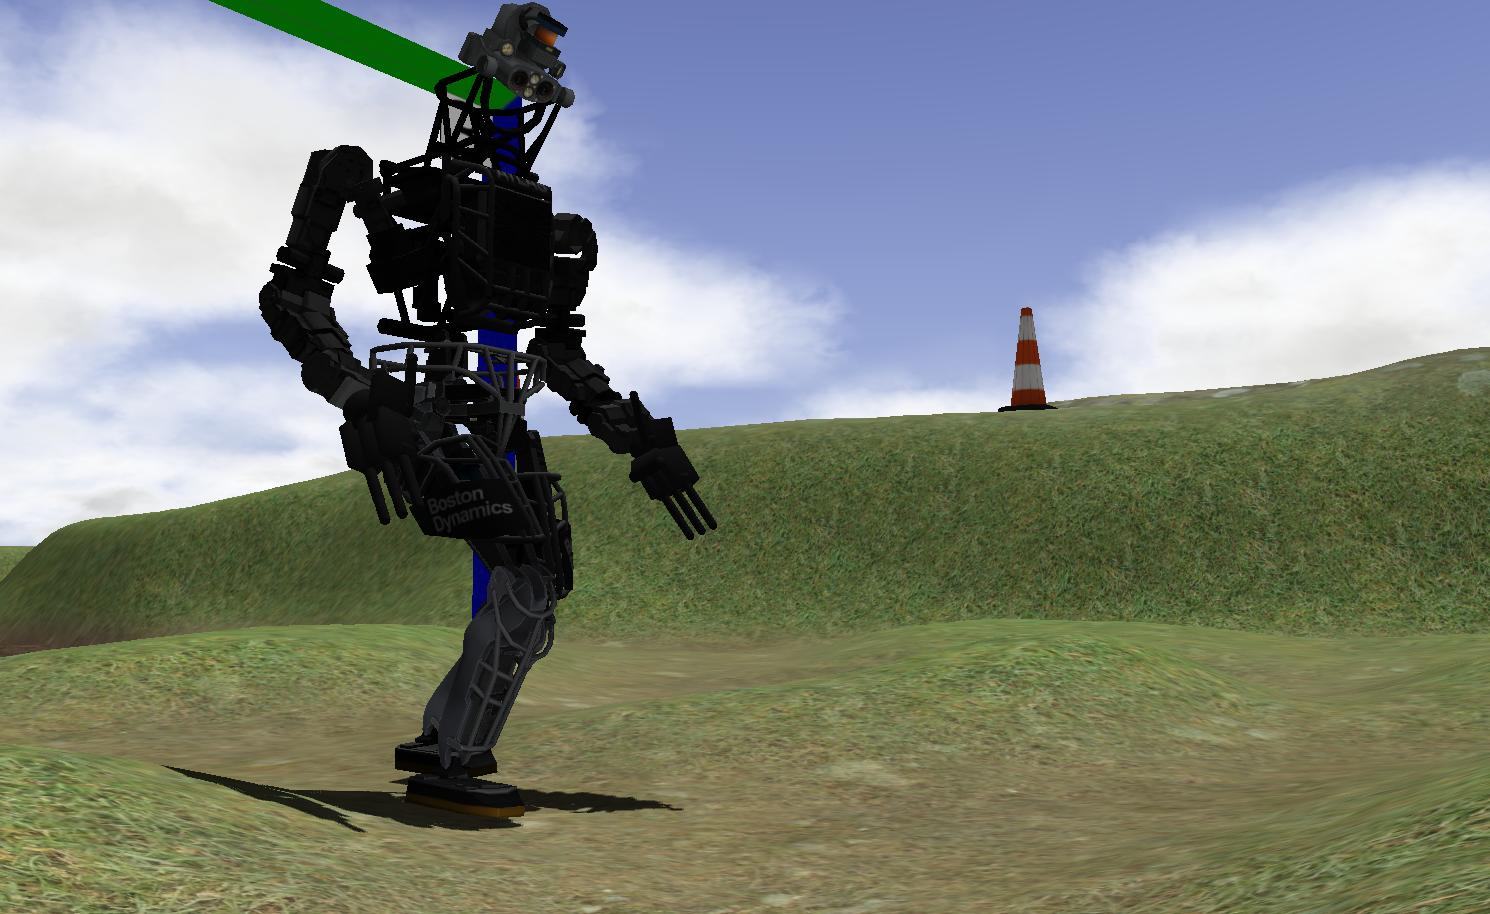
\includegraphics[height=9cm,width=1\textwidth,keepaspectratio]{terrain_assesment/c2_paper.jpg}
              \caption{Задание на пересеченной местности в конкурсе виртуальной робототехники DARPA}
              \label{fig:terrain_assesment/c2_paper.jpg}
          \end{figure}
          
    \item Оценка местности в соответствии с возможностями робота. Она основывается на перепаде высот, который может преодолеть робот. Если робот не может его преодолеть, значит, местность неудовлетворительная \cite{hung_Advanced_2004,Howard2000} \pic{fig:terrain_assesment/c3_paper.png}.
          
          \begin{figure}[H]
              \centering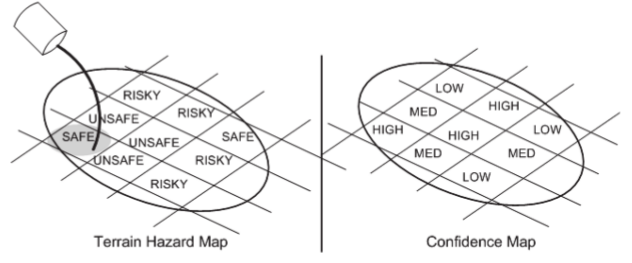
\includegraphics[height=6cm,width=1\textwidth,keepaspectratio]{terrain_assesment/c3_paper.png}
              \caption{Пример карт местности: карта опасности местности и карта достоверности местности}
              \label{fig:terrain_assesment/c3_paper.png}
          \end{figure}

    \item Оценка по карте с использованием ряда анализируемых параметров, таких как дисперсия, дальность, тип почвенно-растительного покрова, количество граней и так далее \cite{hung_Advanced_2004}.
    \item Получение искусственных поверхностей на основе параметров генерации. Первая версия этой идеи была связана с получением жестких ландшафтов с квадратной сеткой, где каждая ячейка имеет некоторую высоту \cite{sancho-pradel_Survey_2010} \pic{fig:terrain_assesment/c1_paper.png}.
          
          \begin{figure}[H]
              \centering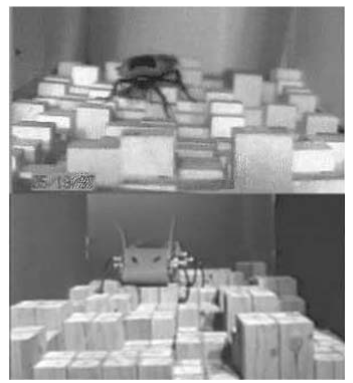
\includegraphics[height=10cm,width=1\textwidth,keepaspectratio]{terrain_assesment/c1_paper.png}
              \caption{Рельеф с параметризованными ячейками}
              \label{fig:terrain_assesment/c1_paper.png}
          \end{figure}
\end{enumerate}

Рассмотрев преимущества и недостатки всех вариантов, последний подход с некоторыми модификациями и расширениями лучше всего подходит для оценки сложности поверхности.

\section{Обзор алгоритмов триангуляций}
Для решения задачи построения карты с помощью тактильного очувствления генерировать поверхность на основе полученных точек является адекватным решением, так как большинство алгоритмов навигации используют облака точек в своих данных. Таким образом концепты, используемые в других алгоритмах, могут быть адаптированны и в данной задаче. Эта задача формулируется следующим образом. Необходимо получить поверхность из набора точек, полученных с ног робота. Одним из примеров оболочки является выпуклая оболочка. Выпуклая оболочка это наименьшее выпуклое множество, содержащее в себе некоторое множество $X$.

Для выбора алгоритма необходимо формализовать ограничения и условия, которые присутствуют в конкретной задаче по построению карты с помощью тактильного очувствления \cite{ebertInterpolationExtrapolationComparison2014,kumarSurfaceTriangulationSurvey,aurenhammerVoronoiDiagramsSurvey1991}.
\begin{itemize}
    \item Граница вокруг объекта должна быть вогнутой формы, а не выпуклой. Более подробно этот тезис объясняется в главе \nameref{ch:ch4}.
    \item Плотность полученного облака точек не играет роли, так как разрабатываемый алгоритм не будет страдать из-за разряженности точек.
\end{itemize}

Область интерполяции \cite{brooksCharacterizingDomainRegression1988,patelLinearProgramDetect1995,baranyiEffectsParameterizationPerformance1996,haffnerEscapingConvexHull2001,kingDangersExtremeCounterfactuals2006} --- это когда одна группа объектов или набор данных является базой для определения диапазона значений для интерполяции и заключена в некую границу выпуклой формы. Область за пределами этой границы или корпуса обозначается как область экстраполяции. Обычно эту область называют выпуклой оболочкой.

Существуют множество алгоритмов, которые рассматривают случай, когда у одной группы объектов оболочка не является выпуклой. \cite{rejerHypertubePossibleInterpolation2006,j.a.leonardUsingRadialBasis1992,verleysenLearningHighdimensionalData2001}.

Для решения задачи построения карты необходимо использовать алгоритмы, основанные на получении вогнутой оболочки. Чаще всего такие алгоритмы используют за основу выпуклую оболочку и модифицируют ее.

Первыми алгоритмами для вычисления выпуклых оболочек были Алгоритм Грэхема \cite{grahamEfficientAlgorithDetermining1972} и Алгоритм Джарвиса \cite{jarvisIdentificationConvexHull1973}, которые были усовершенствованы в \cite{chanOptimalOutputsensitiveConvex1996}.

Для получения выпуклой оболочки большей размерности был предложен алгоритм быстрой оболочки \cite{clarksonApplicationsRandomSampling1988}.Более современные алгоритмы применимы к более комплексным областям применения. К примеру такими алгоритмами являются <<динамические выпуклые оболочки>>, <<аппроксимация оболочки для больших наборов данных>>, <<алгоритмы выпуклых оболочек для больших размерностей>> \cite{brodalDynamicPlanarConvex2002,khosravaniSimpleAlgorithmConvex2013,zhongFindingConvexHull2014}. Например для задач построения карты для беспилотных автомобилей требуется решения в режиме реально времени, авторы разрабатывают усовершенствования производительности алгоритмов путем распараллеливания и использования графического процессора (GPU) для определения внутренних точек \cite{zhongFindingConvexHull2014,cintraSpeculativeParallelizationRandomized2004,cintraSpeculativeParallelizationRandomized2004,tangSMI2012Full2012,tzengFindingConvexHulls2012}.

Для построения вогнутых оболочек существует несколько различных подходов к вычислению границ произвольной формы. Основные концепции алгоритмов построения вогнутых оболочек основаны на методах ближайших соседей, kernel функциях или триангуляции Делоне. Хотя это не совсем алгоритм для построения вогнутой оболочки, существует также подход, который с помощью статистики определяет признаки новизны. В итоге данный подход решает ту же проблему \cite{zhongFindingConvexHull2014}. 

Известным алгоритмом для построения вогнутой оболочки является $\alpha$-shapes \cite{edelsbrunnerShapeSetPoints1983,edelsbrunnerThreedimensionalAlphaShapes1992}. Это обобщение вогнутой оболочки, где $\alpha$ - параметр, и по мере приближения $\alpha$ к 0, $\alpha$-оболочка приближается к обычной выпуклой оболочке. $\alpha$-оболочки строятся из диаграмм Вороного. Есть альтернатива --- $\chi$-фигуры \cite{duckhamEfficientGenerationSimple2008}. Алгоритм $\chi$-форм является простым, гибким и эффективным для построения возможно невыпуклого простого многоугольника, который характеризует форму набора входных точек на плоскости, называемую характерной формой. Вместо диаграмм Вороного алгоритм основан на триангуляции точек по методу Делоне. Есть еще модификации на основанные на алгоритме Грэхема \cite{xuConcaveHullAlgorithm2010} с унаследованными ограничениями.  Другой подход представлен Парком \cite{parkNewConcaveHull2012}, который начинается с выпуклой оболочки и применяет алгоритм "копания". 

Благодаря работе \cite{j.a.leonardUsingRadialBasis1992} и  метода машинного обучения  SVM, возник новый класс методов обнаружения. Однако одноклассовые SVM не дают точной оболочки, и для различения между внутренним и внешним необходимо задать порог. С дополнительной информацией возможна двухклассовая SVM. 

Для вычисления независимых оболочек для нескольких групп объектов предлагается алгоритм с использованием алгоритма кластеризации общих ближайших соседей (SNN) , который вычисляет оболочку для каждой группы, применяя подход k-nearest neighbors (kNN) \cite{moreiraConcaveHullKnearest2007,ertozNewSharedNearest2002,chauBorderSamplesDetection2011,xiaBORDEREfficientComputation2006}.

\section{Обзор разработанной системы}
\begin{figure}[H]
    \centering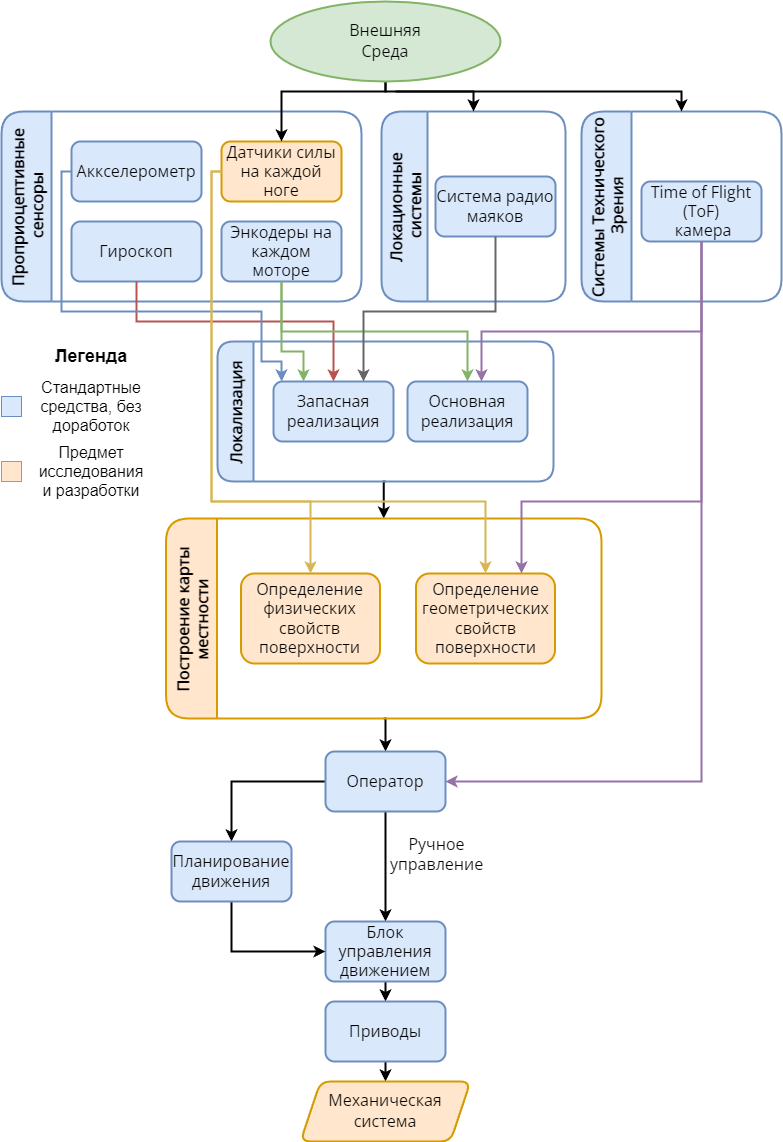
\includegraphics[height=22cm,width=1\textwidth,keepaspectratio]{main_diag.drawio.png}
    \caption{Структурная схема разработанной системы}
    \label{fig:diag_system.png}
\end{figure}

Для реализации экспериментальных исследований разработана робототехническая система, структурная схема которой показана выше \pic{fig:diag_system.png}

Оранжевым цветом выделены те компоненты системы, которые представляют собой предмет исследования в рамках диссертационной работы. Их разработка и научная новизна описаны в последующих главах диссертации. Голубым цветом выделены блоки, соответствующие которым элементы в разработанную систему были интегрированы как стандартные средства,   без каких-либо существенных доработок.

Верхний блок --- внешняя среда, то есть вся информация о внешнем мире, с которой работает робот. То есть, это окружающее робота пространство, которое возможно считывать с помощью установленных сенсоров, с ним возможно физически взаимодействовать.

Следующая группа блоков связана с сенсорами. Здесь представлены <<Проприоцептивные сенсоры>>, то есть внутренние датчики, такие как гироскоп, акселерометр, энкодеры и датчики силы. Единственному оранжевому соответствующему элементу в данной группе <<Датчики силы на каждой ноге>> посвящена глава \nameref{ch:ch3}. В ней рассказывается о разработке датчика на основе Velostat, о проблемах, возникающих при использовании данного материала, и как эти проблемы были решены.

Также есть группа блоков, посвященная техническому зрению. В представленном роботе это камеры Time of Flight (ToF). Это камера, которая может выдавать облако точек. Это другое облако точек, не то, которое получено с ног робота, но их возможно объединить для получения более точной карты местности.

Последней группой элементов является <<Локационные системы>>, представленные системой радио маяков. Во время движения робот может оставлять радио маяки, таким образом делая радио локационную сеть. Такая сеть позволяет определять местоположение робота в пространстве. Предметом исследования эта задача не является.

Ниже находится следующая группа блоков <<Локализация>>. Она основана на данных, полученных с сенсоров. В данной группе расположены два блока <<Основная реализация>> и <<Запасная реализация>>. Первая является более точной. Она может быть реализована на основе системы радио маяков или с помощью системы технического зрения. Но самый точный результат может быть получен при объединении двух систем. Запасная реализация является резервной, когда отказала основная реализация, или когда та выдает некорректные результаты. Она основана на Инерциальном измерительном устройстве (IMU), датчиках силы и системе маяков.

В рамках диссертационного исследования были разработаны следующая группа блоков <<Построение модели местности>> был реализован и разработан автором диссертации. Она состоит из трех блоков: <<Определение физических свойств поверхности>>, <<Построение карты местности>>, <<Определение геометрических свойств поверхности>>. Первый блок позволяет параллельно с исследованием геометрических свойств поверхности, посредством ее пальпирования, определять материал по которому ходит робот. Построение карты местности объединяет данные с других двух блоков и выводит результат в машино и человеко читабельные виды. Более подробно данная группа описана в главе \nameref{ch:ch4}.

Полученные данные попадают оператору, и оператор может управлять роботом, как в ручном режиме, так и просто задав область, куда роботу нужно прийти. Эта высокоуровневая команда передается в блок управления движением, которая в последствии преобразуется в низкоуровневые команды для приводов робота. С помощью данных команд, механическая система, представленная разработанным роботом приводится в движение и выполняется поставленная оператором задача.

В работе научная новизна представлена в элементах схемы, связанных с очувствлением: датчики силы, построение карты местности, определение физических свойств объекта.

\section{Применимость системы}
Необходимо понимать возможности робототехнической системы. Следующей задачей является формализация условий ее применимости. Из полученных условий возможно определить конкретные существующие места, где такую систему возможно применить.

Итогом размышлений на тему возможностей был сделан вывод, что данная система может использоваться в узких пещерах, где не может пролезть человек. Шагающие машины обладают лучшей проходимостью, чем гусеничный или колесный тип движителя, поэтому его использования в местах, где есть большой перепад высот и нет возможности набирать высокую скорость из-за обилия препятствий обоснован. Для получения геометрической поверхности разработан алгоритм создания вогнутой оболочки с помощью триангуляции Делоне и alpha геометрии. На входе этот алгоритм использует облако точек, полученное с педипуляторов робота. Физические свойства поверхности определяются с помощью обучения стендовой установки на различных типах поверхности с использованием алгоритма SVM и kNN.